% Options for packages loaded elsewhere
\PassOptionsToPackage{unicode}{hyperref}
\PassOptionsToPackage{hyphens}{url}
\documentclass[
  ignorenonframetext,
  aspectratio=169,
]{beamer}
\newif\ifbibliography
\usepackage{pgfpages}
\setbeamertemplate{caption}[numbered]
\setbeamertemplate{caption label separator}{: }
\setbeamercolor{caption name}{fg=normal text.fg}
\beamertemplatenavigationsymbolsempty
% remove section numbering
\setbeamertemplate{part page}{
  \centering
  \begin{beamercolorbox}[sep=16pt,center]{part title}
    \usebeamerfont{part title}\insertpart\par
  \end{beamercolorbox}
}
\setbeamertemplate{section page}{
  \centering
  \begin{beamercolorbox}[sep=12pt,center]{section title}
    \usebeamerfont{section title}\insertsection\par
  \end{beamercolorbox}
}
\setbeamertemplate{subsection page}{
  \centering
  \begin{beamercolorbox}[sep=8pt,center]{subsection title}
    \usebeamerfont{subsection title}\insertsubsection\par
  \end{beamercolorbox}
}
% Prevent slide breaks in the middle of a paragraph
\widowpenalties 1 10000
\raggedbottom
\AtBeginPart{
  \frame{\partpage}
}
\AtBeginSection{
  \ifbibliography
  \else
    \frame{\sectionpage}
  \fi
}
\AtBeginSubsection{
  \frame{\subsectionpage}
}
\usepackage{iftex}
\ifPDFTeX
  \usepackage[T1]{fontenc}
  \usepackage[utf8]{inputenc}
  \usepackage{textcomp} % provide euro and other symbols
\else % if luatex or xetex
  \usepackage{unicode-math} % this also loads fontspec
  \defaultfontfeatures{Scale=MatchLowercase}
  \defaultfontfeatures[\rmfamily]{Ligatures=TeX,Scale=1}
\fi
\usepackage{lmodern}
\ifPDFTeX\else
  % xetex/luatex font selection
\fi
% Use upquote if available, for straight quotes in verbatim environments
\IfFileExists{upquote.sty}{\usepackage{upquote}}{}
\IfFileExists{microtype.sty}{% use microtype if available
  \usepackage[]{microtype}
  \UseMicrotypeSet[protrusion]{basicmath} % disable protrusion for tt fonts
}{}
\makeatletter
\@ifundefined{KOMAClassName}{% if non-KOMA class
  \IfFileExists{parskip.sty}{%
    \usepackage{parskip}
  }{% else
    \setlength{\parindent}{0pt}
    \setlength{\parskip}{6pt plus 2pt minus 1pt}}
}{% if KOMA class
  \KOMAoptions{parskip=half}}
\makeatother
\usepackage{longtable,booktabs,array}
\usepackage{caption}
\captionsetup[table]{skip=6pt}
\newcounter{none} % for unnumbered tables
\usepackage{calc} % for calculating minipage widths
\usepackage{caption}
% Make caption package work with longtable
\makeatletter
\def\fnum@table{\tablename~\thetable}
\makeatother
\usepackage{graphicx}
\makeatletter
\newsavebox\pandoc@box
\newcommand*\pandocbounded[1]{% scales image to fit in text height/width
  \sbox\pandoc@box{#1}%
  \Gscale@div\@tempa{\textheight}{\dimexpr\ht\pandoc@box+\dp\pandoc@box\relax}%
  \Gscale@div\@tempb{\linewidth}{\wd\pandoc@box}%
  \ifdim\@tempb\p@<\@tempa\p@\let\@tempa\@tempb\fi% select the smaller of both
  \ifdim\@tempa\p@<\p@\scalebox{\@tempa}{\usebox\pandoc@box}%
  \else\usebox{\pandoc@box}%
  \fi%
}
% Set default figure placement to htbp
\def\fps@figure{htbp}
\makeatother
\setlength{\emergencystretch}{3em} % prevent overfull lines
\providecommand{\tightlist}{%
  \setlength{\itemsep}{0pt}\setlength{\parskip}{0pt}}
% Auto-generated by infrastructure/rendering/_pdf_latex_helpers.py::extract_math_font_preamble.
% Minimal header passed to Pandoc via -H so Beamer slides pick up the same math font
% as the combined-PDF path. Adjust the manuscript's preamble.md to change the font globally.
\usepackage{unicode-math}
\setmathfont{latinmodern-math.otf}

% Manuscript macro/package fallbacks (newcommand -> providecommand).
% Core mathematics
\usepackage{amsmath}
\usepackage{amssymb}
% Document layout
% Tables
\usepackage{booktabs}
% Caption styling (booktabs already loaded above). Small caption font with a
% bold label ("Figure 1", "Table 2") gives the math/figure-heavy layout a
% consistent, journal-like caption rhythm without fighting pandoc-crossref —
% pandoc emits standard \caption{}, and caption/captionsetup only restyle it.
% ── Theorem environments ─────────────────────────────────────────────────
% amsthm is loaded above. The FedGVI<->Friston bridge is stated as a small
% number of theorems/definitions/lemmas/propositions/corollaries; sharing one
% counter (definition/lemma/proposition/corollary all step the `theorem`
% counter) gives a single monotone numbering 1, 2, 3, ... across all kinds, so
% authors can reference them as Theorem 1, Definition 2, Corollary 3 without a
% per-kind counter drifting out of order. Plain style for theorem-like results,
% definition style (upright body) for definitions.
% (algorithm2e intentionally not loaded: this manuscript states results as
% numbered amsthm Theorems/Definitions, not algorithm2e pseudocode.)
% Code listings
\usepackage{listings}
% Typography and formatting
% (siunitx intentionally not loaded: no \SI/\num units appear in this manuscript.)
% Cross-references and citations
% (cleveref and titlesec intentionally not loaded: unavailable in this TeX tree
% and not required. Cross-references resolve through pandoc-crossref's own
% \ref-style names — no \cref appears — and section heading styling falls back
% to the pandoc/LaTeX defaults.)
% ── TeX Live Basic-compatible mono font for code listings ────────────
% Latin Modern Mono is bundled with TeX Live Basic and keeps the manuscript
% renderable on minimal TeX installations. Mathematical Unicode coverage is
% provided separately by Latin Modern Math below, so the code font does not
% need a private JuliaMono installation.
%
% Use the TeX font filename rather than the system-family name: the minimal
% TeX Live fontconfig database may not register the OpenType family even though
% kpsewhich can resolve the bundled files.
% Math font for unicode-math: Latin Modern Math (TeX Live) has full BMP
% coverage including U+2223 (\mid), U+226A/226B (\ll/\gg), and the Greek/
% blackboard letters used in equations. Without an explicit \setmathfont,
% unicode-math falls back to lmroman text font which lacks several glyphs
% and emits "Missing character" warnings on every \mid in math mode.

% Slide layout defaults for warning-clean scientific decks.
\usepackage{etoolbox}
\IfFileExists{xurl.sty}{\usepackage{xurl}}{}
\IfFileExists{seqsplit.sty}{\usepackage{seqsplit}}{\newcommand{\seqsplit}[1]{#1}}
\protected\def\breakseq#1{\seqsplit{#1}}
\protected\def\breaktt#1{\begingroup\ttfamily\seqsplit{#1}\endgroup}
\setlength{\emergencystretch}{6em}
\tolerance=5000
\hbadness=10000
\hfuzz=1pt
\setlength{\tabcolsep}{2pt}
\AtBeginEnvironment{longtable}{\tiny\renewcommand{\arraystretch}{0.86}\setlength{\tabcolsep}{1pt}}
\AtBeginEnvironment{tabular}{\tiny\renewcommand{\arraystretch}{0.86}\setlength{\tabcolsep}{1pt}}
\AtBeginEnvironment{equation}{\tiny}
\AtBeginEnvironment{equation*}{\tiny}
\AtBeginEnvironment{align}{\tiny}
\AtBeginEnvironment{align*}{\tiny}
\AtBeginEnvironment{itemize}{\footnotesize}
\AtBeginEnvironment{enumerate}{\footnotesize}
\AtBeginEnvironment{description}{\footnotesize}
\setbeamerfont{caption}{size=\tiny}
\setbeamerfont{caption name}{size=\tiny}
\setbeamerfont{normal text}{size=\small}
\setbeamerfont{frametitle}{size=\small}
\setbeamerfont{section title}{size=\footnotesize}
\setbeamerfont{subsection title}{size=\footnotesize}
\setbeamertemplate{section page}{%
  \centering
  \begin{beamercolorbox}[sep=12pt,center,wd=\paperwidth]{section title}
    \parbox{0.86\paperwidth}{\centering\usebeamerfont{section title}\insertsection\par}
  \end{beamercolorbox}
}
\setbeamertemplate{subsection page}{%
  \centering
  \begin{beamercolorbox}[sep=8pt,center,wd=\paperwidth]{subsection title}
    \parbox{0.86\paperwidth}{\centering\usebeamerfont{subsection title}\insertsubsection\par}
  \end{beamercolorbox}
}
\setlength{\abovecaptionskip}{2pt}
\setlength{\belowcaptionskip}{0pt}

% Natbib and cross-reference fallbacks — slides don't load natbib
% or cleveref, but combined-PDF manuscript prose may emit these
% commands. The fallback renders citations as a bracketed key list
% and cross-references as detokenized labels so slides don't fail on
% undefined control sequences or raw underscores. \providecommand is
% a no-op if packages load later.
\providecommand{\citep}[1]{[#1]}
\providecommand{\citet}[1]{#1}
\providecommand{\citealp}[1]{#1}
\providecommand{\citeauthor}[1]{#1}
\providecommand{\citeyear}[1]{#1}
\providecommand{\cref}[1]{\texttt{\detokenize{#1}}}
\providecommand{\Cref}[1]{\texttt{\detokenize{#1}}}
\providecommand{\crefrange}[2]{\texttt{\detokenize{#1}}--\texttt{\detokenize{#2}}}
\providecommand{\Crefrange}[2]{\texttt{\detokenize{#1}}--\texttt{\detokenize{#2}}}
\providecommand{\paragraph}[1]{\textbf{#1}\ }

% Opt-in accessible presentation profile.
\setbeamerfont{normal text}{size*={20pt}{24pt}}
\setbeamerfont{frametitle}{size*={28pt}{32pt}}
\setbeamerfont{section title}{size*={28pt}{32pt}}
\setbeamerfont{subsection title}{size*={28pt}{32pt}}
\setbeamerfont{caption}{size*={16pt}{19pt}}
\setbeamerfont{caption name}{size*={16pt}{19pt}}
\setbeamerfont{itemize/enumerate body}{size*={20pt}{24pt}}
\setbeamerfont{itemize/enumerate subbody}{size*={20pt}{24pt}}
\setbeamerfont{itemize/enumerate subsubbody}{size*={20pt}{24pt}}
\setbeamerfont{itemize item}{size*={20pt}{24pt}}
\setbeamerfont{itemize subitem}{size*={20pt}{24pt}}
\setbeamerfont{itemize subsubitem}{size*={20pt}{24pt}}
\setbeamerfont{description body}{size*={20pt}{24pt}}
\setbeamerfont{description item}{size*={20pt}{24pt}}
\setbeamerfont{quote}{size*={20pt}{24pt}}
\setbeamerfont{quotation}{size*={20pt}{24pt}}
\AtBeginEnvironment{longtable}{\fontsize{20pt}{24pt}\selectfont}
\AtBeginEnvironment{tabular}{\fontsize{20pt}{24pt}\selectfont}
\AtBeginEnvironment{equation}{\fontsize{20pt}{24pt}\selectfont}
\AtBeginEnvironment{equation*}{\fontsize{20pt}{24pt}\selectfont}
\AtBeginEnvironment{align}{\fontsize{20pt}{24pt}\selectfont}
\AtBeginEnvironment{align*}{\fontsize{20pt}{24pt}\selectfont}
\AtBeginEnvironment{itemize}{\fontsize{20pt}{24pt}\selectfont}
\AtBeginEnvironment{enumerate}{\fontsize{20pt}{24pt}\selectfont}
\AtBeginEnvironment{description}{\fontsize{20pt}{24pt}\selectfont}
\AtBeginDocument{\usebeamerfont{normal text}}
\newlength{\AFSlideTableWidth}
% The fixed footer reservation is calibrated with the semantic seven-line regular-body budget.
\setbeamertemplate{footline}{%
  \leavevmode\vbox{%
    \hbox{%
      \begin{beamercolorbox}[wd=\paperwidth,ht=16pt,dp=3pt,center]{author in head/foot}%
        \fontsize{16pt}{19pt}\selectfont Untagged PDF derivative \textbar\ \href{../web/index.html}{HTML reader}%
      \end{beamercolorbox}%
    }%
    \vskip6pt%
  }%
}
% Accessible footer reserved height: 25pt.

\newtheorem{proposition}{Proposition}
\newtheorem{hypothesis}{Hypothesis}
\newtheorem{remark}[theorem]{Remark}
\newtheorem{axiom}{Axiom}
\newtheorem{property}{Property}
\usepackage{bookmark}
\IfFileExists{xurl.sty}{\usepackage{xurl}}{} % add URL line breaks if available
\urlstyle{same}
% fallback for those not using the hyperref driver hyperxmp:
\makeatletter
\@ifundefined{xmpquote}{\newcommand{\xmpquote}[1]{#1}}{}
\makeatother
\hypersetup{
  hidelinks,
  pdfcreator={LaTeX via pandoc}}

\author{\texorpdfstring{}{}}
\date{}

\begin{document}

\begin{frame}{Contamination sweep: regime-dependent server behavior
under declared attacks}
\protect\phantomsection\label{sec:results-robustness}
\end{frame}

\begin{frame}[fragile]{Contamination sweep (part 2)}
This experiment compares server presets in one active-inference colony.
Its legacy labels borrow FedGVI client-divergence vocabulary (Mildner et
al. 2025), but the presets are not client losses or divergence theorems.
\texttt{KLD} denotes the standard log-linear pool;
\end{frame}

\begin{frame}[fragile]{Contamination sweep (part 3)}
every other label denotes a \texttt{robust\_aggregate} heuristic
constant in KLD (c=0.00), RKL (c=1.50), AR (c=1.30), beta (c=1.70), rcce
(c=1.60). The estimand is consensus mass \(q(\text{true state})\) under
the declared contamination mechanism.
\end{frame}

\begin{frame}{Contamination sweep (part 4)}
The colony contains 7 sentinels, of which 2 mix their broadcasts toward
a confident-wrong delta at each contamination rate. The comparisons
remain conditional on this fixed world, attack target, and preset grid.
\end{frame}

\begin{frame}{Contamination sweep (part 5)}
The evidence map in fig.~6 locates
these comparisons in the conditional heuristic-server lane. It keeps the
fixed-world matched trials distinct from the seed-level review below and
prevents either result from inheriting client-loss or variational-server
guarantees.
\end{frame}

\begin{frame}[fragile]{Contamination sweep (part 6)}
As the contamination rate rises across
\(\{0, 0.225, 0.45, 0.675, 0.9\}\), the \textbf{standard} (\texttt{KLD})
consensus accuracy degrades monotonically:
\end{frame}

\begin{frame}{Contamination sweep (part 7)}
% template-accessible-table-inset
\begingroup
\setlength{\AFSlideTableWidth}{\textwidth}%
\setlength{\LTleft}{\fill}%
\setlength{\LTright}{\fill}%
\begin{longtable}[]{@{}
  >{\raggedright\arraybackslash}p{(\AFSlideTableWidth - 10\tabcolsep) * \real{0.3421}}
  >{\raggedright\arraybackslash}p{(\AFSlideTableWidth - 10\tabcolsep) * \real{0.1316}}
  >{\raggedright\arraybackslash}p{(\AFSlideTableWidth - 10\tabcolsep) * \real{0.1316}}
  >{\raggedright\arraybackslash}p{(\AFSlideTableWidth - 10\tabcolsep) * \real{0.1316}}
  >{\raggedright\arraybackslash}p{(\AFSlideTableWidth - 10\tabcolsep) * \real{0.1316}}
  >{\raggedright\arraybackslash}p{(\AFSlideTableWidth - 10\tabcolsep) * \real{0.1316}}@{}}
\label{tbl:robustness_sweep}\tabularnewline
\toprule\noalign{}
\begin{minipage}[b]{\linewidth}\raggedright
Contamination rate
\end{minipage} & \begin{minipage}[b]{\linewidth}\raggedright
KLD
\end{minipage} & \begin{minipage}[b]{\linewidth}\raggedright
RKL
\end{minipage} & \begin{minipage}[b]{\linewidth}\raggedright
AR
\end{minipage} & \begin{minipage}[b]{\linewidth}\raggedright
beta
\end{minipage} & \begin{minipage}[b]{\linewidth}\raggedright
rcce
\end{minipage} \\
\midrule\noalign{}
\endfirsthead
\toprule\noalign{}
\begin{minipage}[b]{\linewidth}\raggedright
Contamination rate
\end{minipage} & \begin{minipage}[b]{\linewidth}\raggedright
KLD
\end{minipage} & \begin{minipage}[b]{\linewidth}\raggedright
RKL
\end{minipage} & \begin{minipage}[b]{\linewidth}\raggedright
AR
\end{minipage} & \begin{minipage}[b]{\linewidth}\raggedright
beta
\end{minipage} & \begin{minipage}[b]{\linewidth}\raggedright
rcce
\end{minipage} \\
\midrule\noalign{}
\endhead
0 & 1.000 & 0.997 & 0.998 & 0.996 & 0.996 \\
0.225 & 0.999 & 0.993 & 0.995 & 0.990 & 0.992 \\
0.45 & 0.995 & 0.987 & 0.990 & 0.984 & 0.986 \\
0.675 & 0.975 & 0.985 & 0.989 & 0.981 & 0.983 \\
\bottomrule\noalign{}
\end{longtable}
\endgroup
\end{frame}

\begin{frame}[fragile]{Contamination sweep (part 8)}
As the saboteurs capture more belief mass, \texttt{KLD} falls
monotonically while at least one non-reference preset remains above the
stated accuracy threshold. \textbf{Reference trend:} standard accuracy
degrades monotonically with rate, recorded as Yes.
\end{frame}

\begin{frame}{Contamination sweep (part 9)}
\textbf{Worst-rate display check:} at rate 0.900, at least one
non-reference preset remains at or above 0.50, recorded as Yes. Standard
accuracy is 0.6928; the highest robust consensus mass in this
single-world mechanistic sweep is 0.9880, attained by AR.
\end{frame}

\begin{frame}{Contamination sweep (part 10)}
The rate trend above is one deterministic sweep per cell. The paired
profile reruns each rate over \(n_{\rm trial} = 960\) matched trials
nested within the fixed seeded world. Each non-reference preset is
compared with the standard pool, and p-values are BH-adjusted within
method (Benjamini and Hochberg 1995).
\end{frame}

\begin{frame}{Contamination sweep (part 11)}
This is a finite, rate-resolved diagnostic, not a continuous-family
result.
\end{frame}

\begin{frame}{Contamination sweep (part 12)}
% template-accessible-table-inset
\begingroup
\setlength{\AFSlideTableWidth}{\textwidth}%
\setlength{\LTleft}{\fill}%
\setlength{\LTright}{\fill}%
\begin{longtable}[]{@{}
  >{\raggedright\arraybackslash}p{(\AFSlideTableWidth - 6\tabcolsep) * \real{0.2500}}
  >{\raggedright\arraybackslash}p{(\AFSlideTableWidth - 6\tabcolsep) * \real{0.1500}}
  >{\raggedright\arraybackslash}p{(\AFSlideTableWidth - 6\tabcolsep) * \real{0.3750}}
  >{\raggedright\arraybackslash}p{(\AFSlideTableWidth - 6\tabcolsep) * \real{0.2250}}@{}}
\label{tbl:paired-by-rate}\tabularnewline
\toprule\noalign{}
\begin{minipage}[b]{\linewidth}\raggedright
Server preset
\end{minipage} & \begin{minipage}[b]{\linewidth}\raggedright
Rate
\end{minipage} & \begin{minipage}[b]{\linewidth}\raggedright
Rank-biserial-derived \(d\)-equivalent
\end{minipage} & \begin{minipage}[b]{\linewidth}\raggedright
Label
\end{minipage} \\
\midrule\noalign{}
\endfirsthead
\toprule\noalign{}
\begin{minipage}[b]{\linewidth}\raggedright
Server preset
\end{minipage} & \begin{minipage}[b]{\linewidth}\raggedright
Rate
\end{minipage} & \begin{minipage}[b]{\linewidth}\raggedright
Rank-biserial-derived \(d\)-equivalent
\end{minipage} & \begin{minipage}[b]{\linewidth}\raggedright
Label
\end{minipage} \\
\midrule\noalign{}
\endhead
RKL & 0 & saturated (r=-1) & large \\
\bottomrule\noalign{}
\end{longtable}
\endgroup
\end{frame}

\begin{frame}{Contamination sweep (part 13)}
% template-accessible-table-inset
\begingroup
\setlength{\AFSlideTableWidth}{\textwidth}%
\setlength{\LTleft}{\fill}%
\setlength{\LTright}{\fill}%
\begin{longtable}[]{@{}
  >{\raggedright\arraybackslash}p{(\AFSlideTableWidth - 8\tabcolsep) * \real{0.2564}}
  >{\raggedright\arraybackslash}p{(\AFSlideTableWidth - 8\tabcolsep) * \real{0.1538}}
  >{\raggedright\arraybackslash}p{(\AFSlideTableWidth - 8\tabcolsep) * \real{0.2051}}
  >{\raggedright\arraybackslash}p{(\AFSlideTableWidth - 8\tabcolsep) * \real{0.2051}}
  >{\raggedright\arraybackslash}p{(\AFSlideTableWidth - 8\tabcolsep) * \real{0.1795}}@{}}
\label{tbl:paired-by-rate-inference}\tabularnewline
\toprule\noalign{}
\begin{minipage}[b]{\linewidth}\raggedright
Server preset
\end{minipage} & \begin{minipage}[b]{\linewidth}\raggedright
Rate
\end{minipage} & \begin{minipage}[b]{\linewidth}\raggedright
Raw p
\end{minipage} & \begin{minipage}[b]{\linewidth}\raggedright
q
\end{minipage} & \begin{minipage}[b]{\linewidth}\raggedright
Reject
\end{minipage} \\
\midrule\noalign{}
\endfirsthead
\toprule\noalign{}
\begin{minipage}[b]{\linewidth}\raggedright
Server preset
\end{minipage} & \begin{minipage}[b]{\linewidth}\raggedright
Rate
\end{minipage} & \begin{minipage}[b]{\linewidth}\raggedright
Raw p
\end{minipage} & \begin{minipage}[b]{\linewidth}\raggedright
q
\end{minipage} & \begin{minipage}[b]{\linewidth}\raggedright
Reject
\end{minipage} \\
\midrule\noalign{}
\endhead
RKL & 0 & 1.11e-158 & 1.85e-158 & Yes \\
RKL & 0.225 & 1.11e-158 & 1.85e-158 & Yes \\
RKL & 0.45 & 1.11e-158 & 1.85e-158 & Yes \\
RKL & 0.675 & 1.88e-155 & 2.35e-155 & Yes \\
\bottomrule\noalign{}
\end{longtable}
\endgroup
\end{frame}

\begin{frame}[fragile]{Contamination sweep (part 14)}
The \texttt{KLD} baseline is excluded from both projections because it
is the standard reference, not a self-contrast. The displayed
\(d\)-equivalent is a rank-biserial-derived transform, not raw Cohen's
\(d\); the signed-saturation marker flags contrasts where the
rank-biserial correlation saturates at \(\pm1\).
\end{frame}

\begin{frame}[fragile]{Contamination sweep (part 15)}
These contrasts decorate the server-side \texttt{robust\_aggregate}
heuristic only.
\end{frame}

\begin{frame}{Contamination sweep (part 16)}
\begin{figure}
\centering
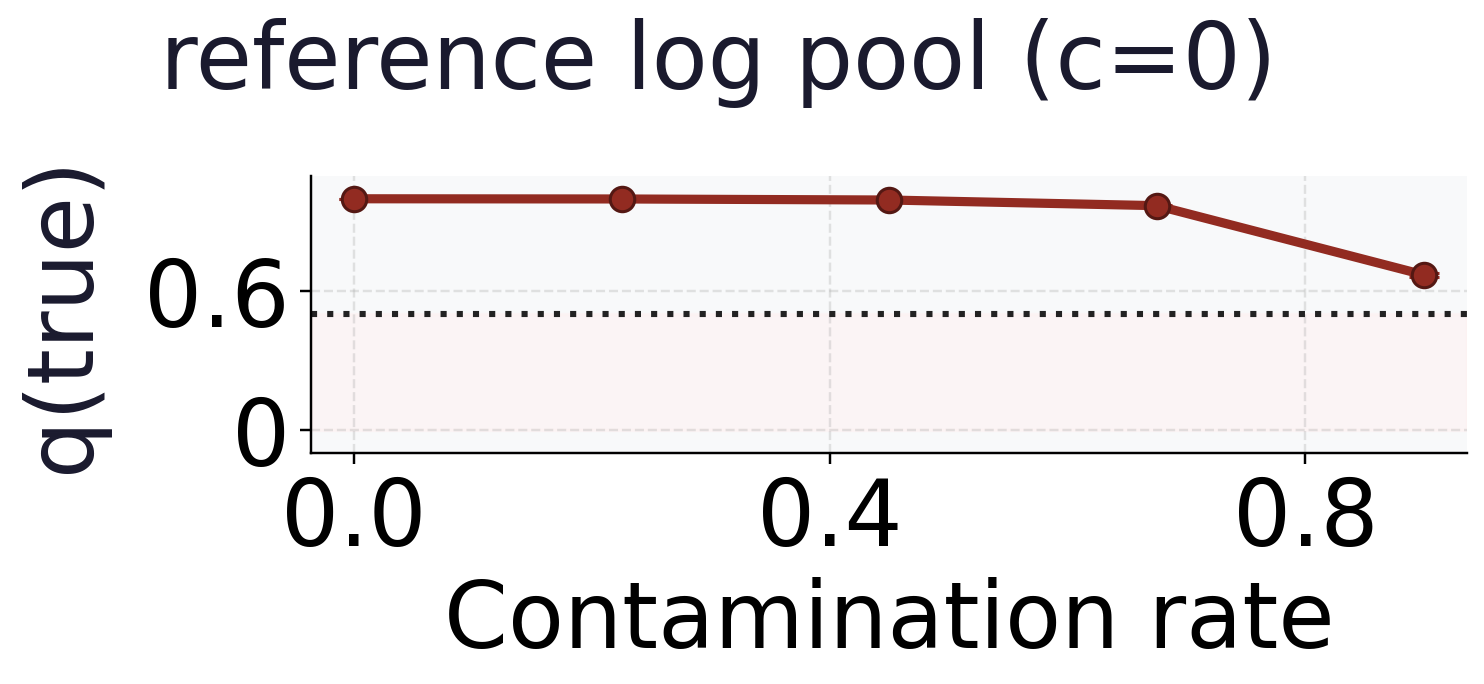
\includegraphics[keepaspectratio,width=0.98\linewidth,height=0.8\textheight,alt={reference log pool (c=0): all configured contamination rates and source-owned uncertainty on a common probability scale.}]{../figures/robustness_sweep.slide-preset-1.png}
\refstepcounter{figure}\label{fig:robustness-sweep-slide-panel-1}
\end{figure}
\end{frame}

\begin{frame}{Contamination sweep (part 17)}
\begin{figure}
\centering
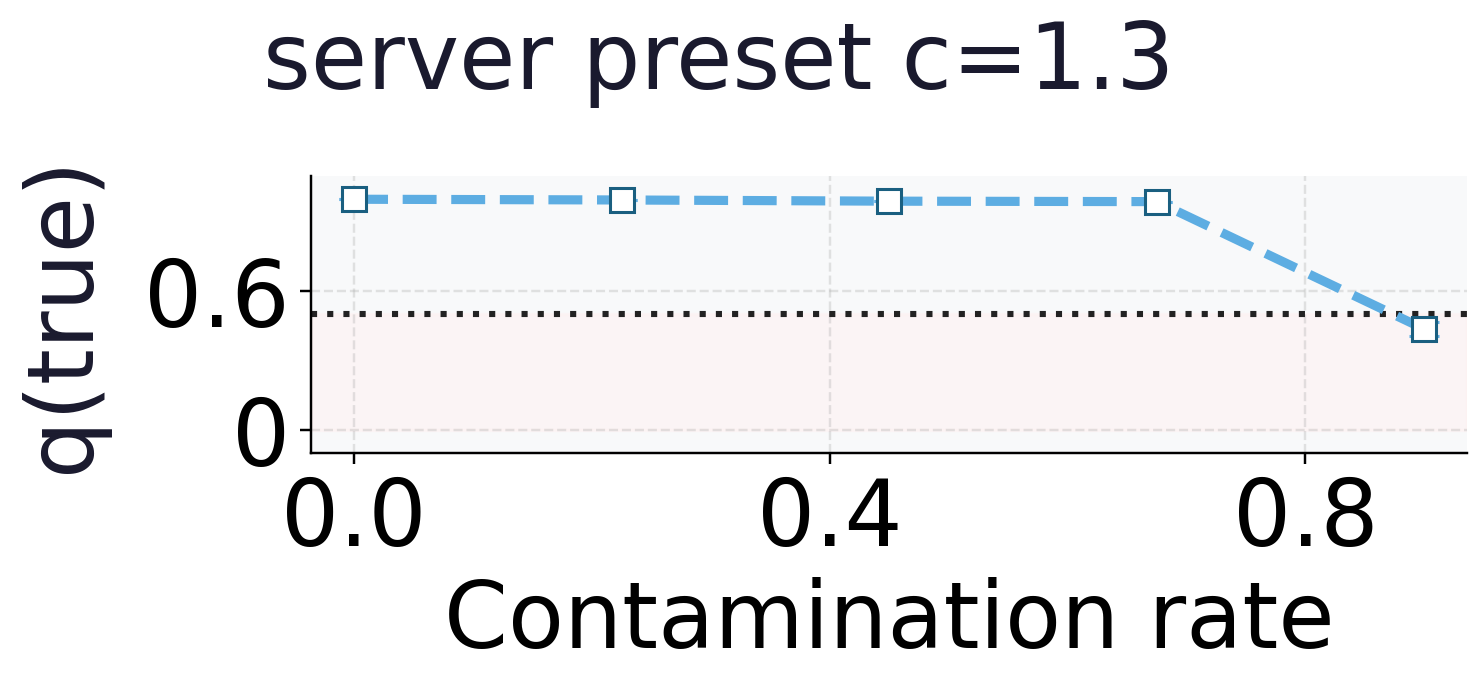
\includegraphics[keepaspectratio,width=0.98\linewidth,height=0.8\textheight,alt={server preset c=1.3: all configured contamination rates and source-owned uncertainty on a common probability scale.}]{../figures/robustness_sweep.slide-preset-2.png}
\refstepcounter{figure}\label{fig:robustness-sweep-slide-panel-2}
\end{figure}
\end{frame}

\begin{frame}{Contamination sweep (part 18)}
\begin{figure}
\centering
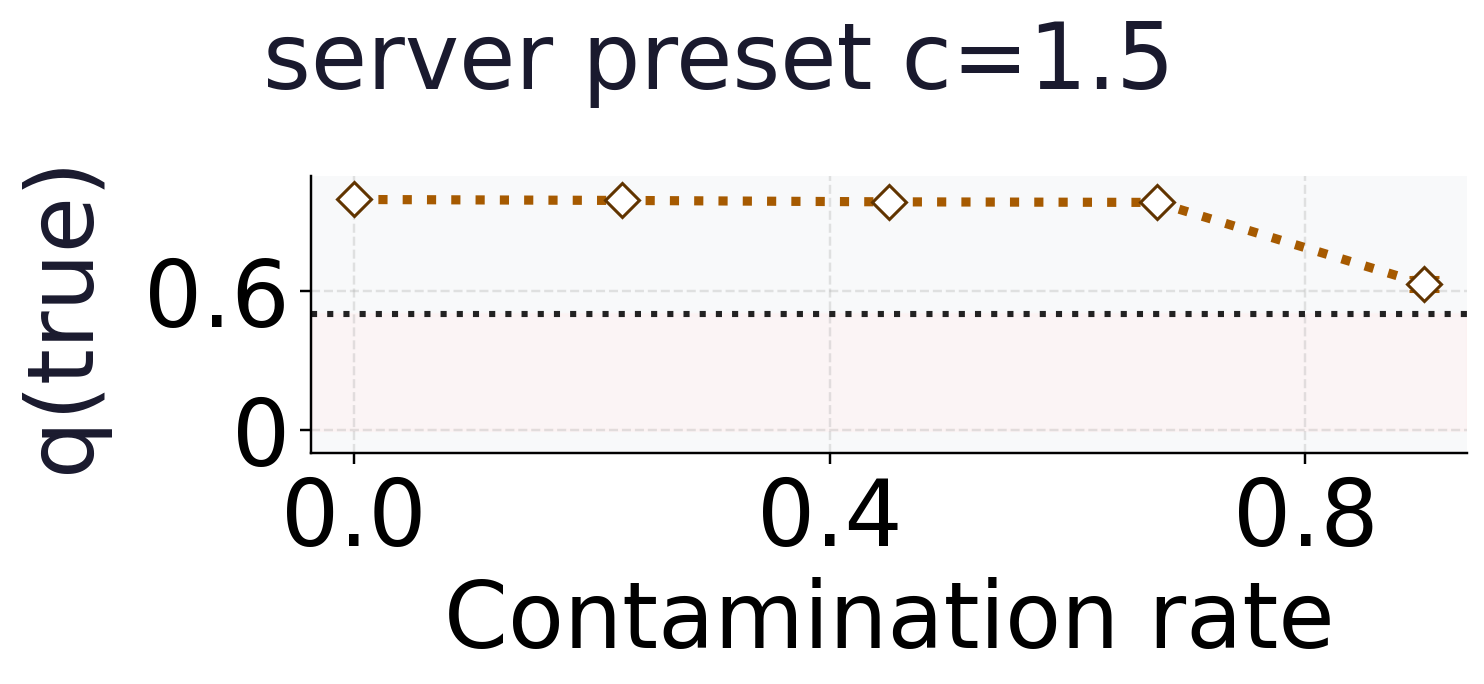
\includegraphics[keepaspectratio,width=0.98\linewidth,height=0.8\textheight,alt={server preset c=1.5: all configured contamination rates and source-owned uncertainty on a common probability scale.}]{../figures/robustness_sweep.slide-preset-3.png}
\refstepcounter{figure}\label{fig:robustness-sweep-slide-panel-3}
\end{figure}
\end{frame}

\begin{frame}{Contamination sweep (part 19)}
\begin{figure}
\centering
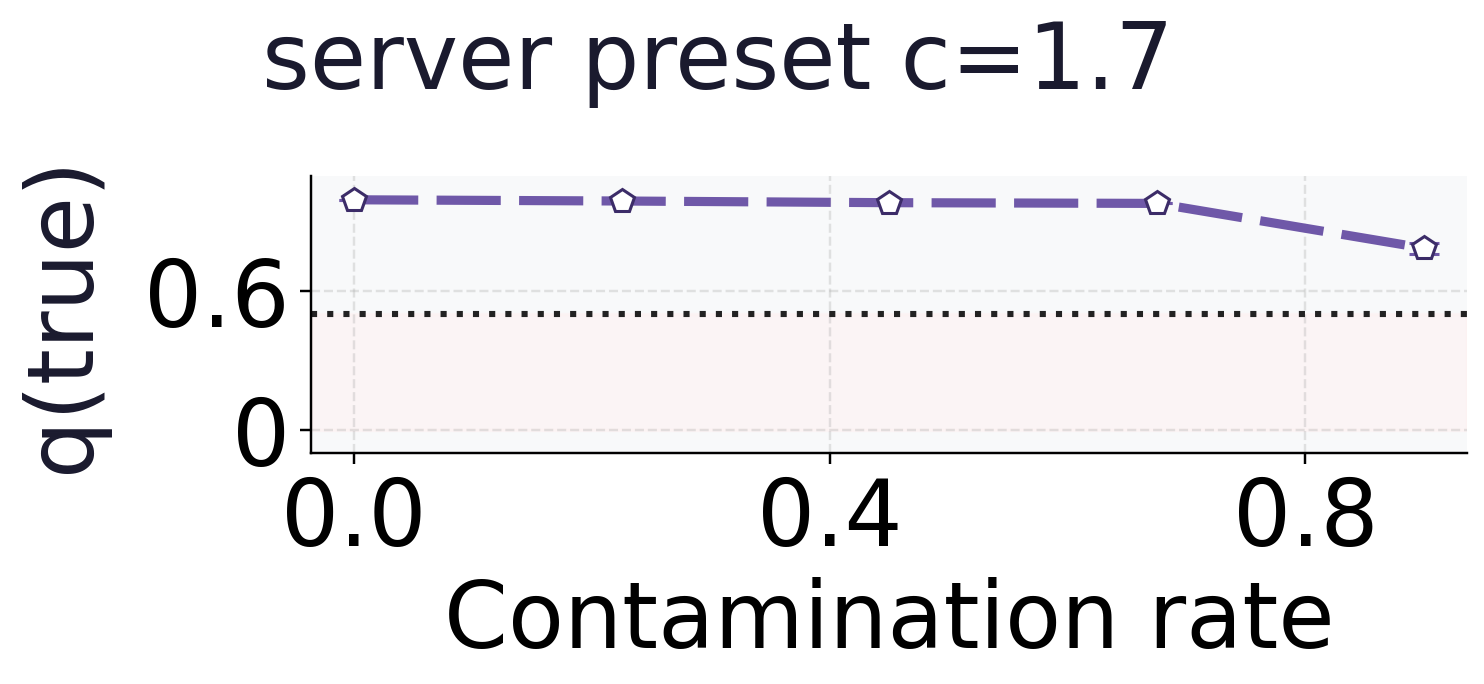
\includegraphics[keepaspectratio,width=0.98\linewidth,height=0.8\textheight,alt={server preset c=1.7: all configured contamination rates and source-owned uncertainty on a common probability scale.}]{../figures/robustness_sweep.slide-preset-4.png}
\refstepcounter{figure}\label{fig:robustness-sweep-slide-panel-4}
\end{figure}
\end{frame}

\begin{frame}{Contamination sweep (part 20)}
\begin{figure}
\centering
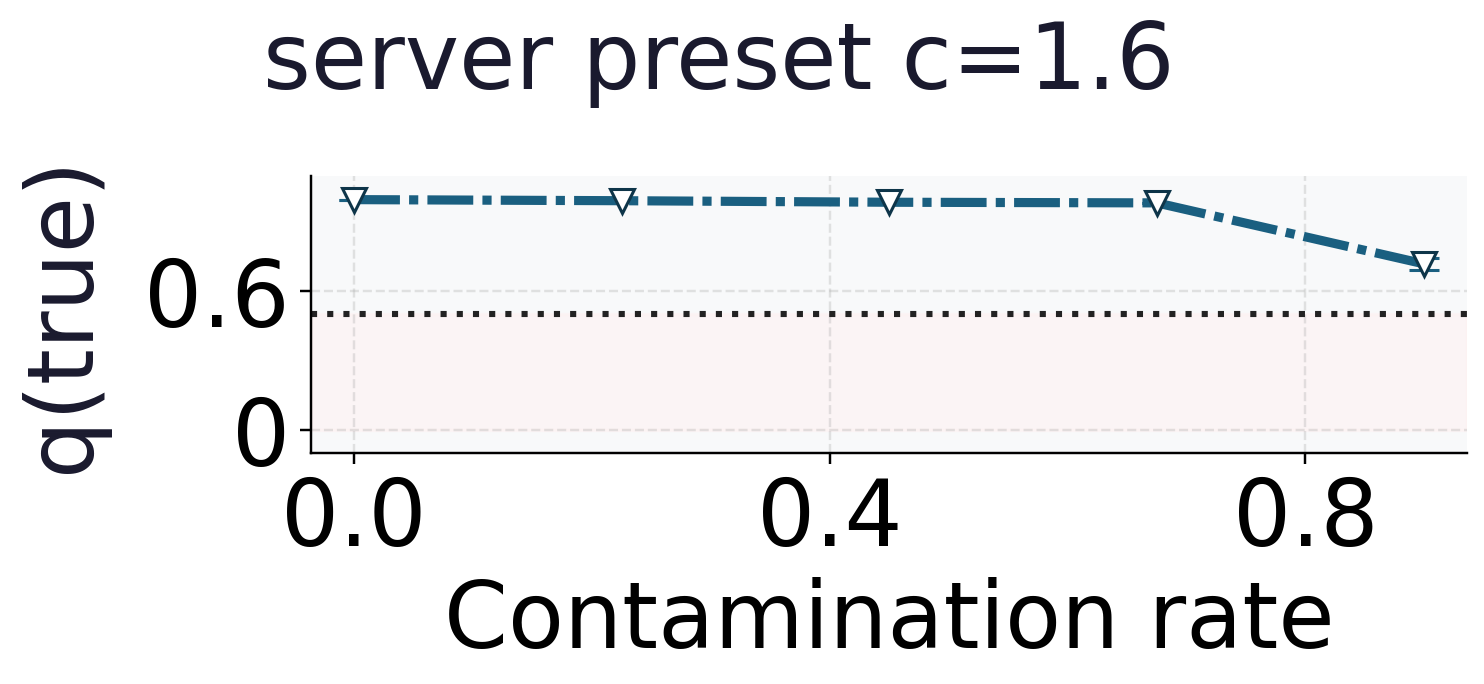
\includegraphics[keepaspectratio,width=0.98\linewidth,height=0.8\textheight,alt={server preset c=1.6: all configured contamination rates and source-owned uncertainty on a common probability scale.}]{../figures/robustness_sweep.slide-preset-5.png}
\refstepcounter{figure}\label{fig:robustness-sweep-slide-panel-5}
\end{figure}
\end{frame}

\begin{frame}{Contamination sweep (part 21)}
\begin{figure}
\centering
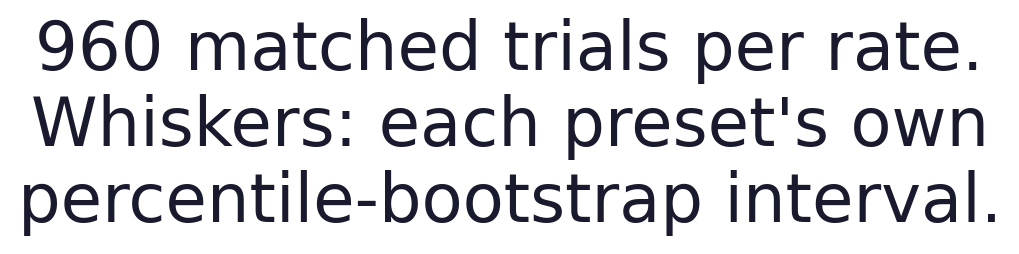
\includegraphics[keepaspectratio,width=0.98\linewidth,height=0.8\textheight,alt={960 matched trials per rate. Whiskers: each preset\textquotesingle s own percentile-bootstrap interval.}]{../figures/robustness_sweep.slide-uncertainty.png}
\refstepcounter{figure}\label{fig:robustness-sweep-slide-panel-6}
\end{figure}
\end{frame}

\begin{frame}{Contamination sweep (part 22)}
\begin{figure}
\centering

\includegraphics[keepaspectratio,width=0.98\linewidth,height=0.8\textheight,alt={Predeclared floor: 0.5. The pale band lies below this reference.}]{../figures/robustness_sweep.slide-threshold.png}
\refstepcounter{figure}\label{fig:robustness-sweep-slide-panel-7}
\end{figure}
\end{frame}

\begin{frame}{Contamination sweep (part 23)}
\begin{figure}
\centering

\includegraphics[keepaspectratio,width=0.98\linewidth,height=0.8\textheight,alt={Largest max-rate preset minus reference: +0.116. Max rate: 0.9.}]{../figures/robustness_sweep.slide-statistics.png}
\refstepcounter{figure}\label{fig:robustness-sweep-slide-panel-8}
\end{figure}
\end{frame}

\begin{frame}{Contamination sweep (part 24)}
\begin{figure}
\centering
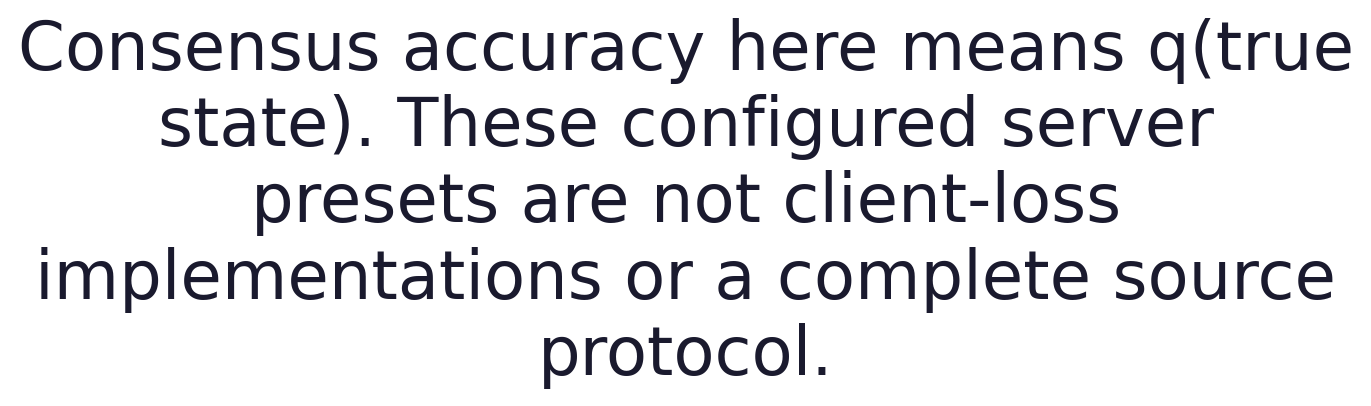
\includegraphics[keepaspectratio,width=0.98\linewidth,height=0.8\textheight,alt={Consensus accuracy here means q(true state). These configured server presets are not client-loss implementations or a complete source protocol.}]{../figures/robustness_sweep.slide-scope.png}
\refstepcounter{figure}\label{fig:robustness-sweep-slide-panel-9}
\end{figure}
\end{frame}

\begin{frame}{Selection-free all-method robustness review}
\protect\phantomsection\label{sec:results-review-grid}
The comparison in fig.~14 is the principal
comparative robustness surface.
\end{frame}

\begin{frame}{Selection-free all-method\ldots{} (part 2)}
It joins the conditional-world cells to the directional rate profiles
while retaining every configured non-reference server preset. It uses
160 deterministic seed replicates and 24 trials nested within each seed
and cell.
\end{frame}

\begin{frame}{Selection-free all-method\ldots{} (part 3)}
Read the portrait surface from top to bottom: Panel A is the full-width
conditional heatmap, and Panels B--D stack the three rate profiles.
Their elbow leaders terminate in reserved right-side label lanes so
curve identity remains separate from the plotted endpoints.
\end{frame}

\begin{frame}{Selection-free all-method\ldots{} (part 4)}
The finite attack union is clean, confident wrong, permutation,
byzantine, drift, label noise, uniform. The rate-resolved directional
mechanisms are confident wrong, byzantine, drift, with entropy controls
uniform, label noise and registered rates
\(\{0, 0.2, 0.4, 0.5, 0.6, 0.7, 0.8, 0.9\}\).
\end{frame}

\begin{frame}{Selection-free all-method\ldots{} (part 5)}
The independent unit is seed within a declared scenario or rate cell;
the nesting rule is n\_trials nested within each seed/cell; no trial is
promoted to an independent world.
\end{frame}

\begin{frame}{Selection-free all-method\ldots{} (part 6)}
The payload is selection-free source payload; every configured non-KLD
method is reported at every directional rate and no winner is used for
inference, and its statistics surface is selection-free. It retains
seed-level contrasts, paired Wilcoxon/rank-biserial results,
percentile-bootstrap intervals, MCSE,
\end{frame}

\begin{frame}{Selection-free all-method\ldots{} (part 7)}
an observed-effect MDE, and BH-adjusted rate families. BH ownership is
BH is applied within each attack-mechanism \texorpdfstring{\ensuremath{\times}}{x} method rate family; cells
sharing design structure are not treated as independent families.
\end{frame}

\begin{frame}{Selection-free all-method\ldots{} (part 8)}
The precision plan targets maximum MCSE 0.0100; the observed maximum is
0.0066 across 96. No method is selected by seed, rate, or pooled mean.
Mixed and reversed cells remain visible, and the grid does not close the
open calibration, external-data, or server-theory questions.
\end{frame}

\begin{frame}{Selection-free all-method\ldots{} (part 9)}
The source-generated exact-value fallback calls the same finite grouping
helper as Panel A. For every displayed attack-by-weight cell it records
the printed grouped mean and the printed half min--max span, preventing
the numeric fallback from drifting from the renderer.
\end{frame}

\begin{frame}{Selection-free all-method\ldots{} (part 10)}
\begin{figure}
\centering
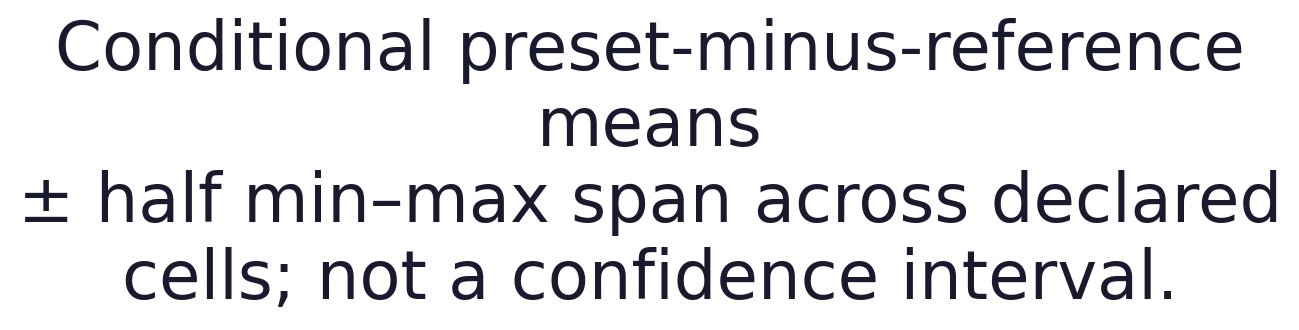
\includegraphics[keepaspectratio,width=0.98\linewidth,height=0.8\textheight,alt={Conditional preset-minus-reference means
± half min--max span across declared cells; not a confidence interval.}]{../figures/robustness_review_grid.slide-conditional-key.png}
\refstepcounter{figure}\label{fig:robustness-review-grid-slide-panel-1}
\end{figure}
\end{frame}

\begin{frame}{Selection-free all-method\ldots{} (part 11)}
\begin{figure}
\centering
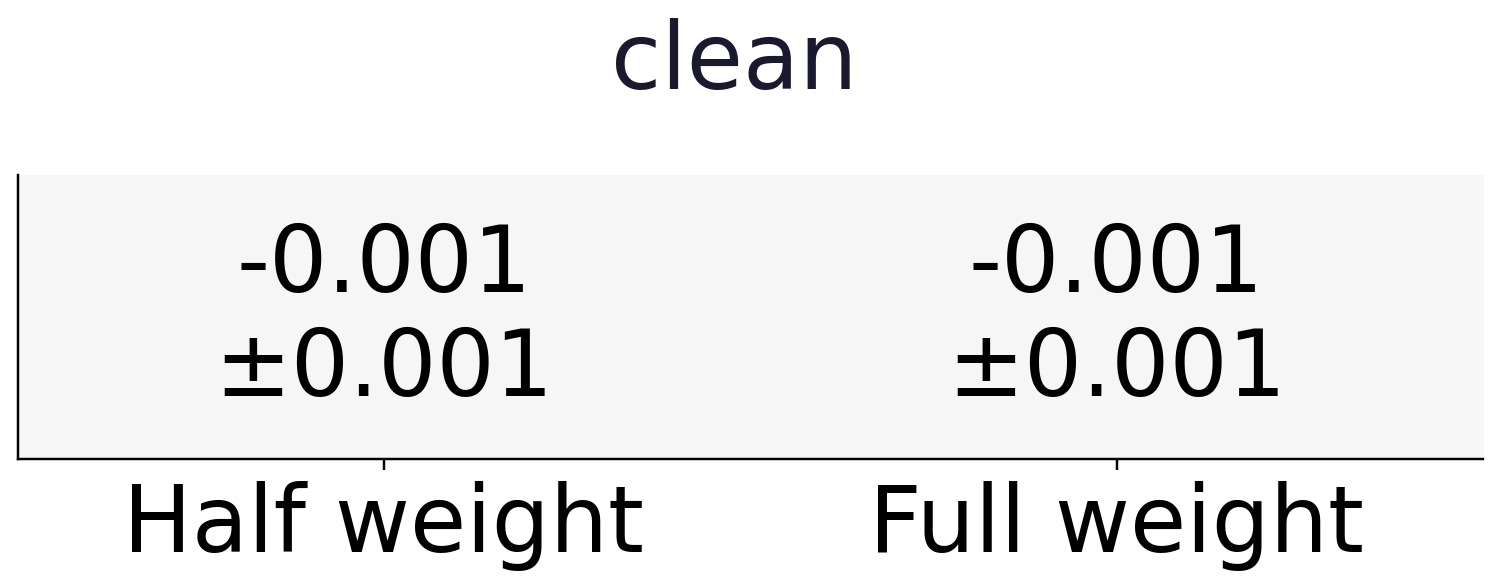
\includegraphics[keepaspectratio,width=0.98\linewidth,height=0.8\textheight,alt={clean: both adversary weights; signed mass means and half min--max spans; common color scale.}]{../figures/robustness_review_grid.slide-conditional-clean.png}
\refstepcounter{figure}\label{fig:robustness-review-grid-slide-panel-2}
\end{figure}
\end{frame}

\begin{frame}{Selection-free all-method\ldots{} (part 12)}
\begin{figure}
\centering
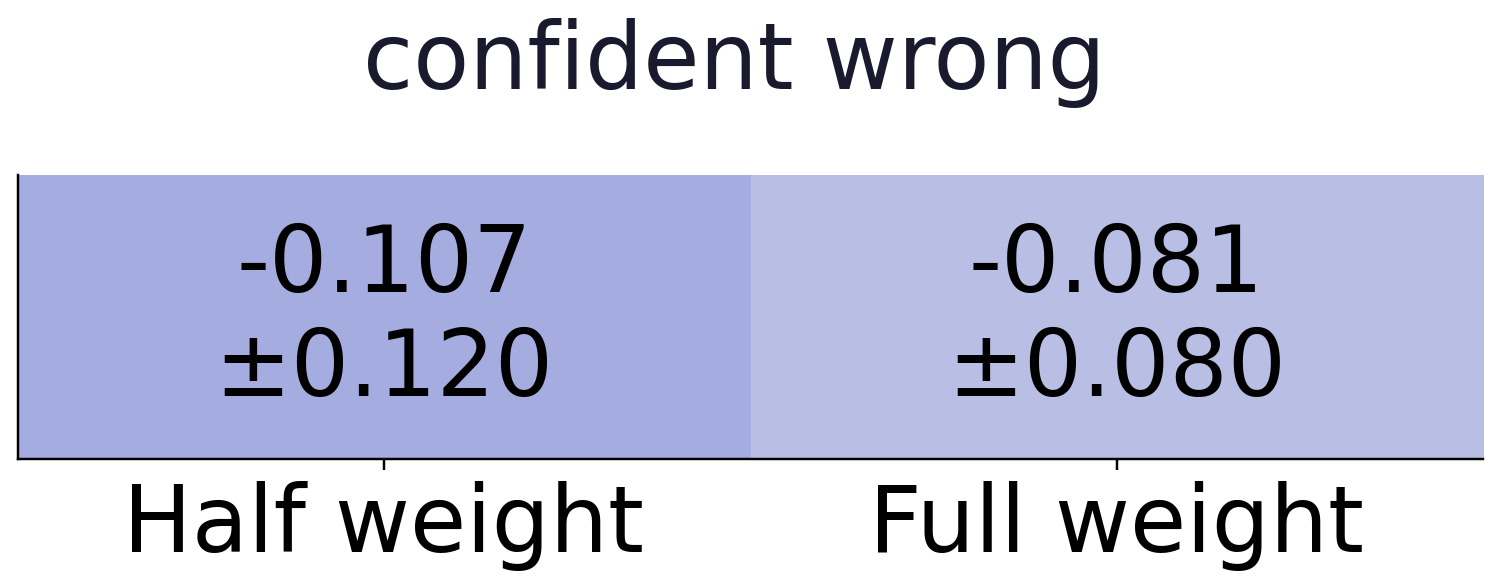
\includegraphics[keepaspectratio,width=0.98\linewidth,height=0.8\textheight,alt={confident wrong: both adversary weights; signed mass means and half min--max spans; common color scale.}]{../figures/robustness_review_grid.slide-conditional-confident-wrong.png}
\refstepcounter{figure}\label{fig:robustness-review-grid-slide-panel-3}
\end{figure}
\end{frame}

\begin{frame}{Selection-free all-method\ldots{} (part 13)}
\begin{figure}
\centering
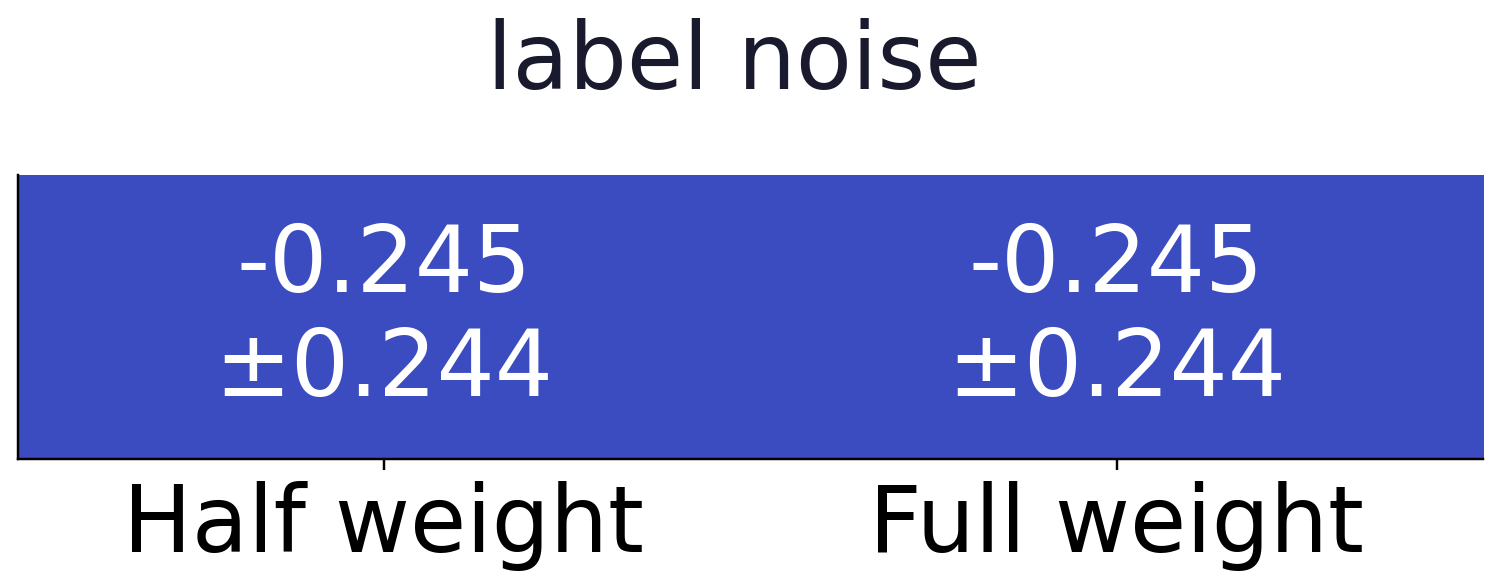
\includegraphics[keepaspectratio,width=0.98\linewidth,height=0.8\textheight,alt={label noise: both adversary weights; signed mass means and half min--max spans; common color scale.}]{../figures/robustness_review_grid.slide-conditional-label-noise.png}
\refstepcounter{figure}\label{fig:robustness-review-grid-slide-panel-4}
\end{figure}
\end{frame}

\begin{frame}{Selection-free all-method\ldots{} (part 14)}
\begin{figure}
\centering
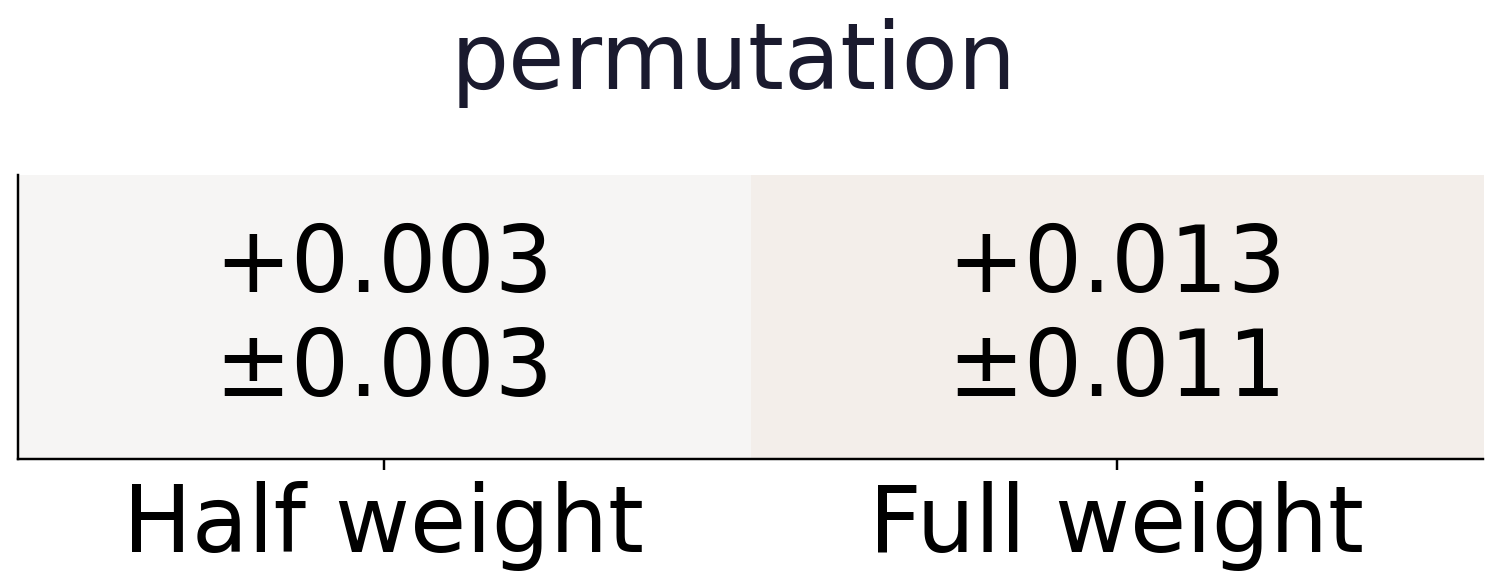
\includegraphics[keepaspectratio,width=0.98\linewidth,height=0.8\textheight,alt={permutation: both adversary weights; signed mass means and half min--max spans; common color scale.}]{../figures/robustness_review_grid.slide-conditional-permutation.png}
\refstepcounter{figure}\label{fig:robustness-review-grid-slide-panel-5}
\end{figure}
\end{frame}

\begin{frame}{Selection-free all-method\ldots{} (part 15)}
\begin{figure}
\centering
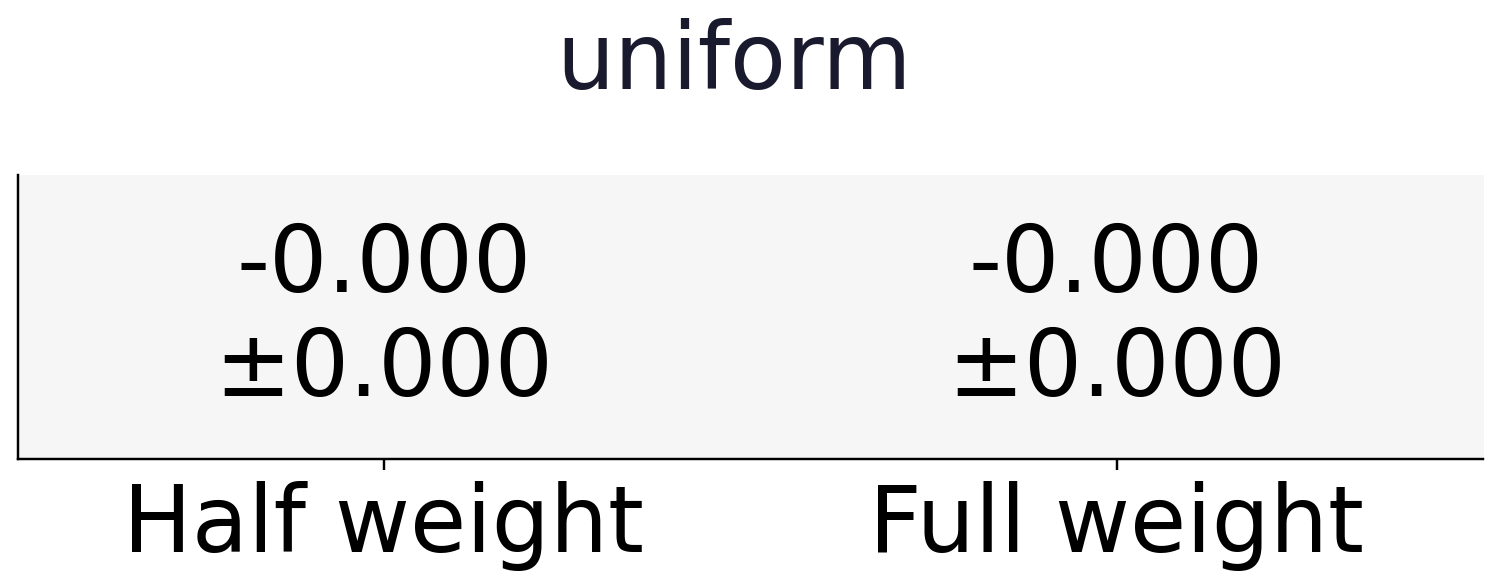
\includegraphics[keepaspectratio,width=0.98\linewidth,height=0.8\textheight,alt={uniform: both adversary weights; signed mass means and half min--max spans; common color scale.}]{../figures/robustness_review_grid.slide-conditional-uniform.png}
\refstepcounter{figure}\label{fig:robustness-review-grid-slide-panel-6}
\end{figure}
\end{frame}

\begin{frame}{Selection-free all-method\ldots{} (part 16)}
\begin{figure}
\centering
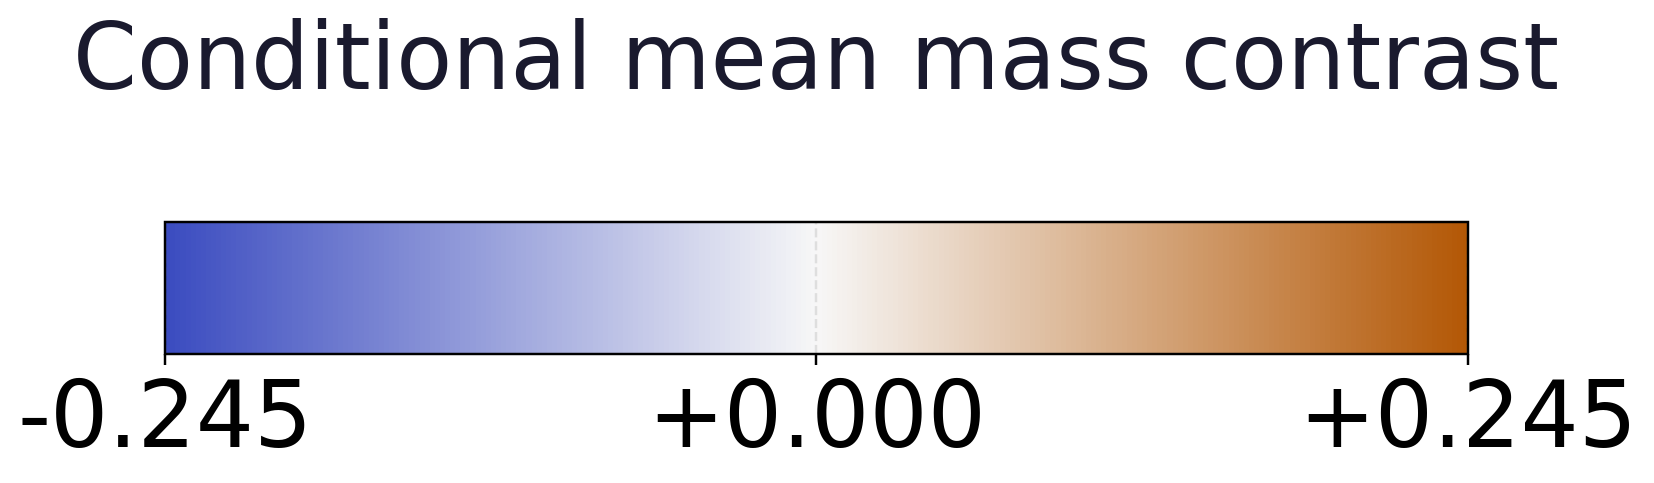
\includegraphics[keepaspectratio,width=0.98\linewidth,height=0.8\textheight,alt={Common signed color scale for every conditional panel; zero is neutral.}]{../figures/robustness_review_grid.slide-conditional-scale.png}
\refstepcounter{figure}\label{fig:robustness-review-grid-slide-panel-7}
\end{figure}
\end{frame}

\begin{frame}{Selection-free all-method\ldots{} (part 17)}
\begin{figure}
\centering
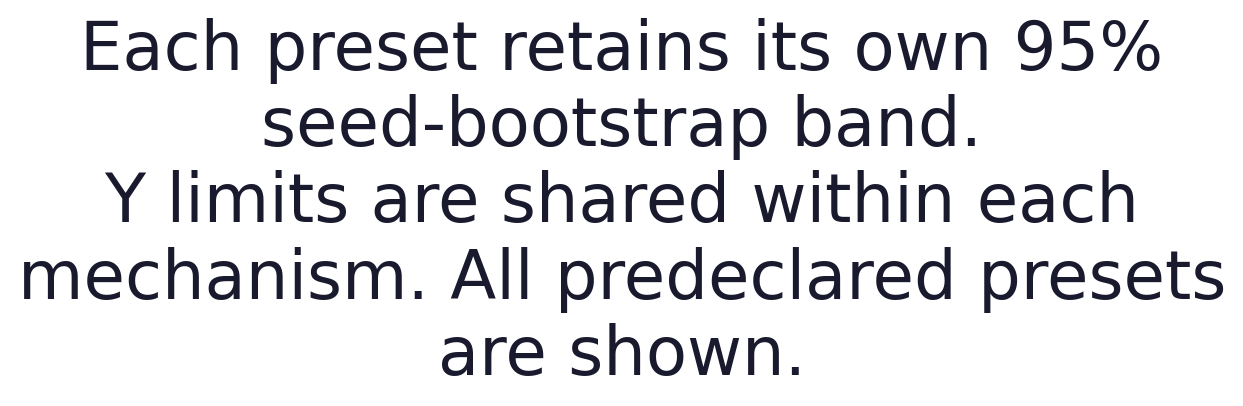
\includegraphics[keepaspectratio,width=0.98\linewidth,height=0.8\textheight,alt={Each preset retains its own 95\% seed-bootstrap band.
Y limits are shared within each mechanism. All predeclared presets are shown.}]{../figures/robustness_review_grid.slide-directional-key.png}
\refstepcounter{figure}\label{fig:robustness-review-grid-slide-panel-8}
\end{figure}
\end{frame}

\begin{frame}{Selection-free all-method\ldots{} (part 18)}
\begin{figure}
\centering
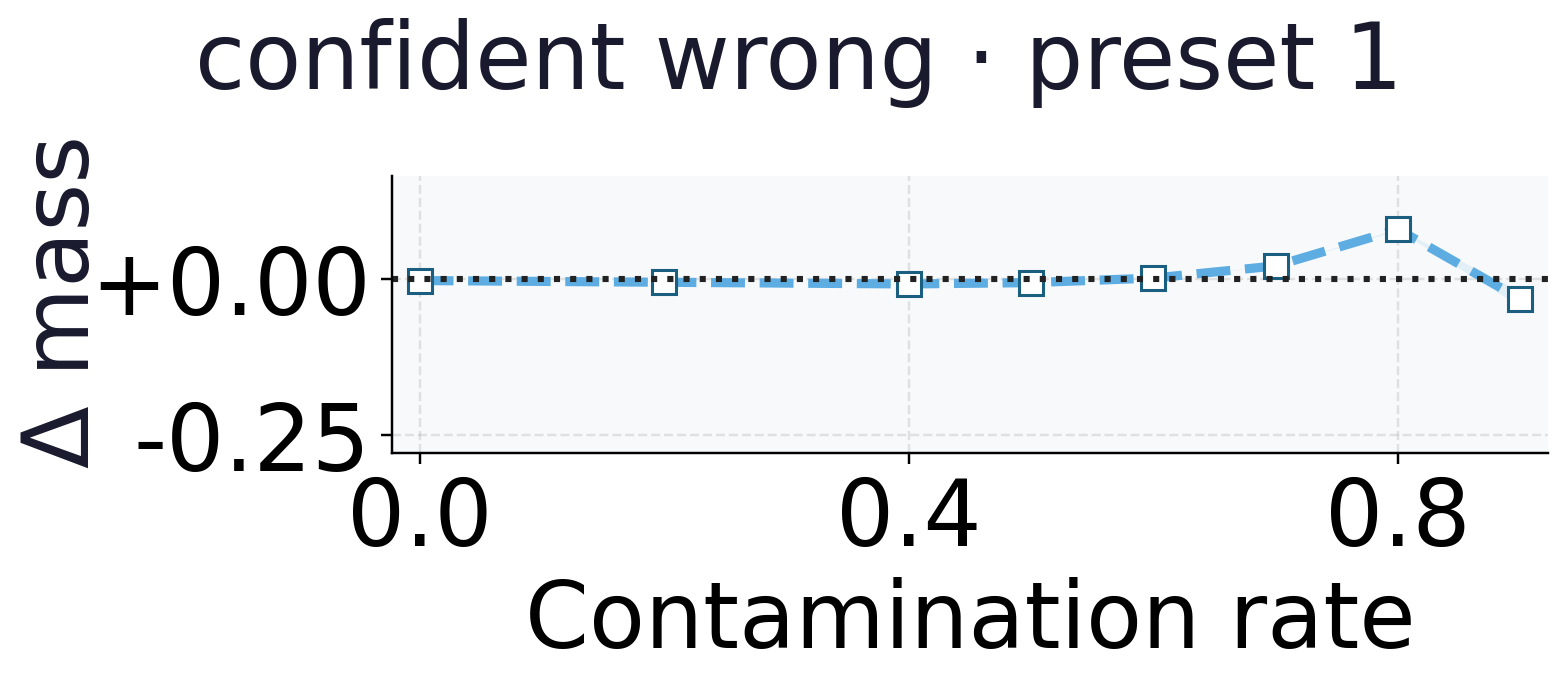
\includegraphics[keepaspectratio,width=0.98\linewidth,height=0.8\textheight,alt={confident wrong, preset 1 (RKL): signed mass contrast and its own 95\% seed-bootstrap band; shared mechanism limits.}]{../figures/robustness_review_grid.slide-directional-confident-wrong-rkl.png}
\refstepcounter{figure}\label{fig:robustness-review-grid-slide-panel-9}
\end{figure}
\end{frame}

\begin{frame}{Selection-free all-method\ldots{} (part 19)}
\begin{figure}
\centering
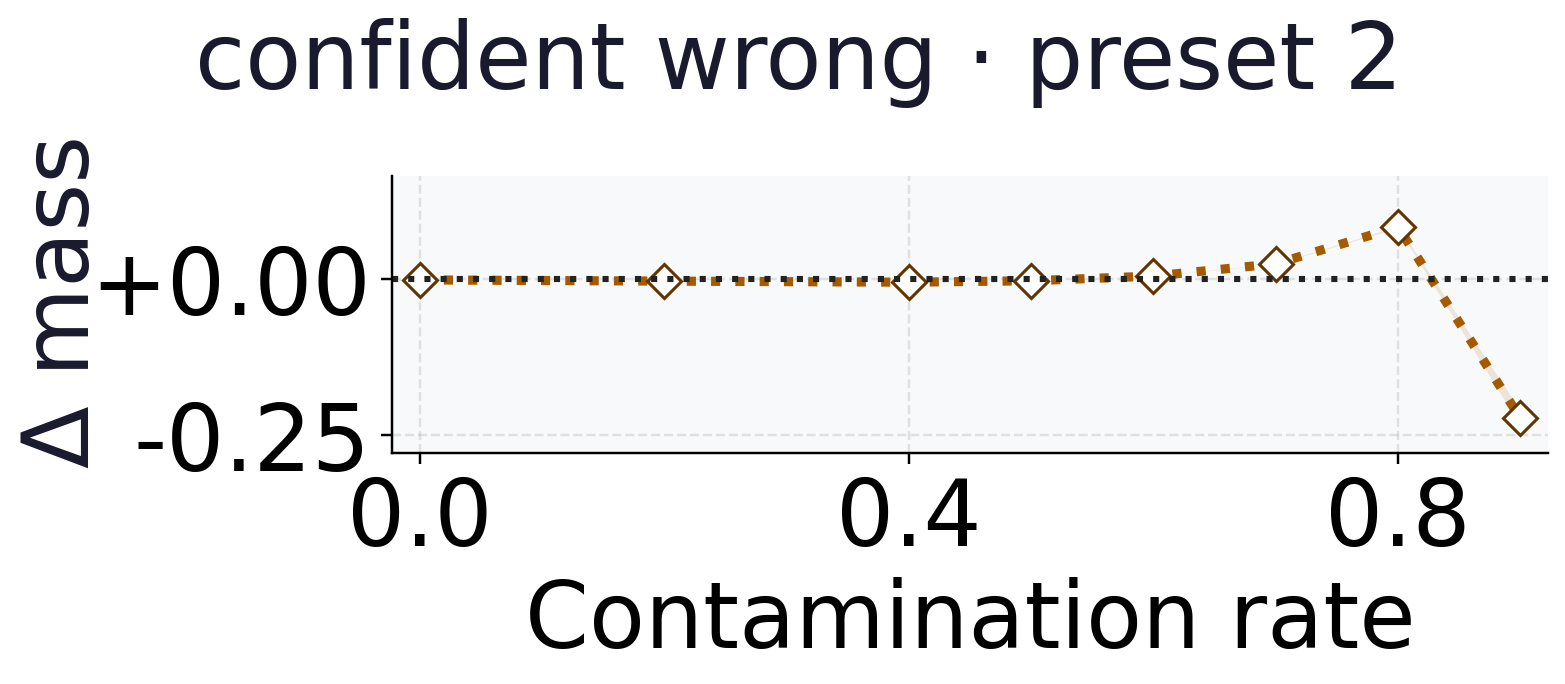
\includegraphics[keepaspectratio,width=0.98\linewidth,height=0.8\textheight,alt={confident wrong, preset 2 (AR): signed mass contrast and its own 95\% seed-bootstrap band; shared mechanism limits.}]{../figures/robustness_review_grid.slide-directional-confident-wrong-ar.png}
\refstepcounter{figure}\label{fig:robustness-review-grid-slide-panel-10}
\end{figure}
\end{frame}

\begin{frame}{Selection-free all-method\ldots{} (part 20)}
\begin{figure}
\centering
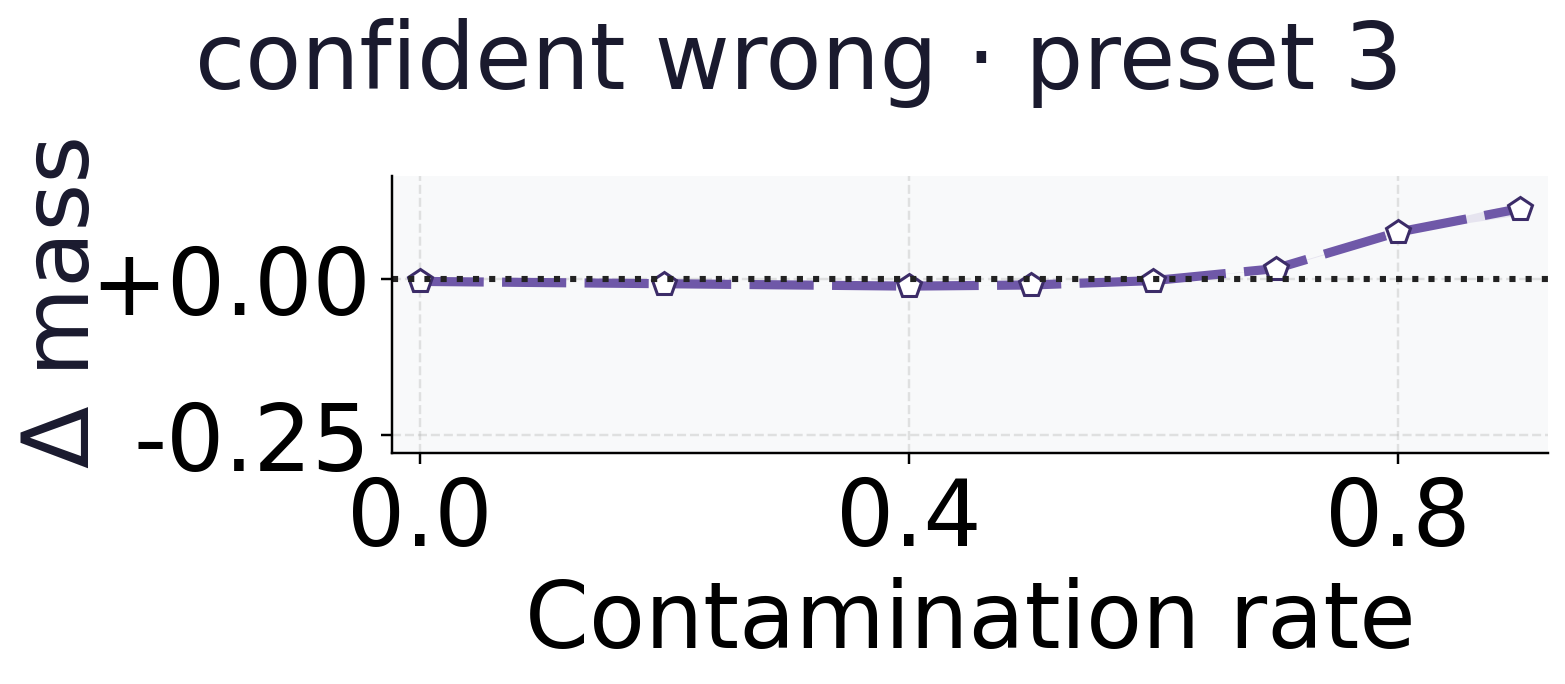
\includegraphics[keepaspectratio,width=0.98\linewidth,height=0.8\textheight,alt={confident wrong, preset 3 (beta): signed mass contrast and its own 95\% seed-bootstrap band; shared mechanism limits.}]{../figures/robustness_review_grid.slide-directional-confident-wrong-beta.png}
\refstepcounter{figure}\label{fig:robustness-review-grid-slide-panel-11}
\end{figure}
\end{frame}

\begin{frame}{Selection-free all-method\ldots{} (part 21)}
\begin{figure}
\centering
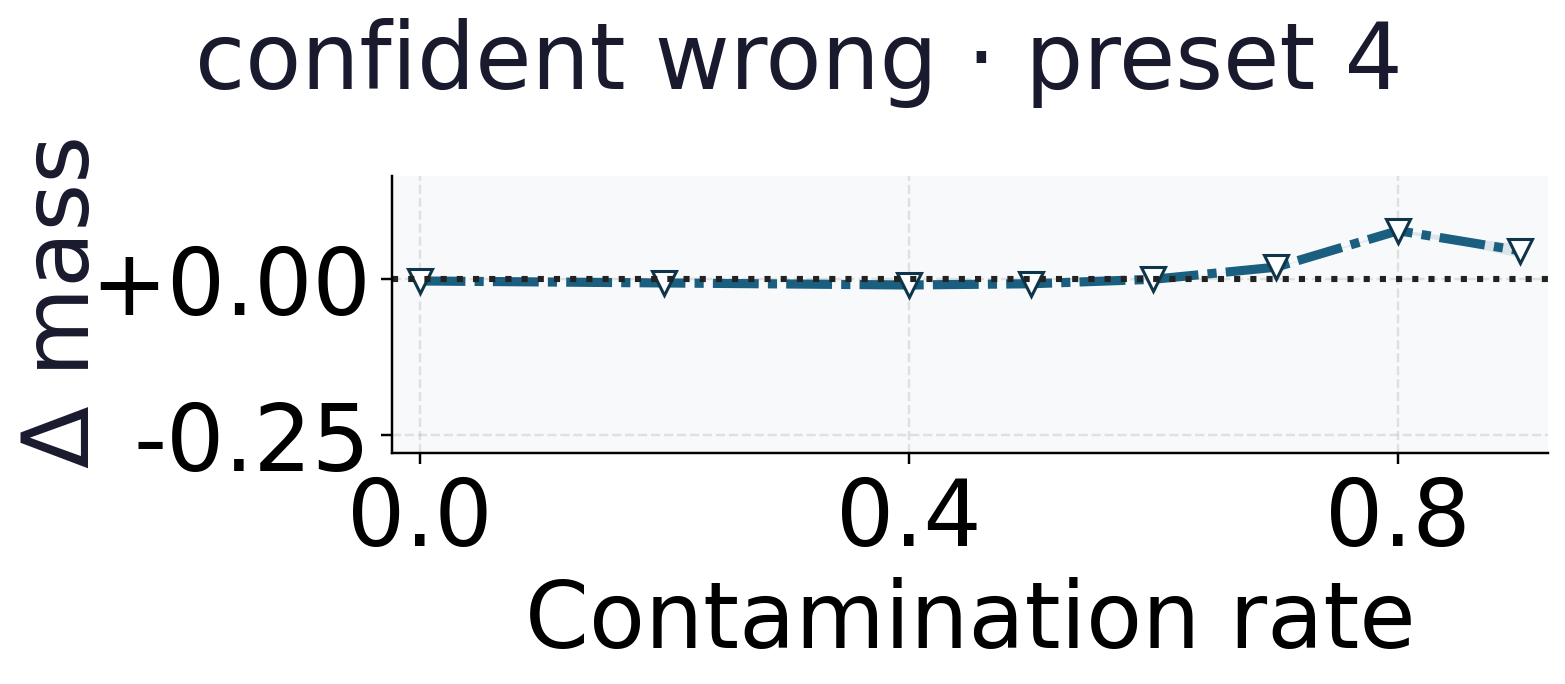
\includegraphics[keepaspectratio,width=0.98\linewidth,height=0.8\textheight,alt={confident wrong, preset 4 (rcce): signed mass contrast and its own 95\% seed-bootstrap band; shared mechanism limits.}]{../figures/robustness_review_grid.slide-directional-confident-wrong-rcce.png}
\refstepcounter{figure}\label{fig:robustness-review-grid-slide-panel-12}
\end{figure}
\end{frame}

\begin{frame}{Selection-free all-method\ldots{} (part 22)}
\begin{figure}
\centering
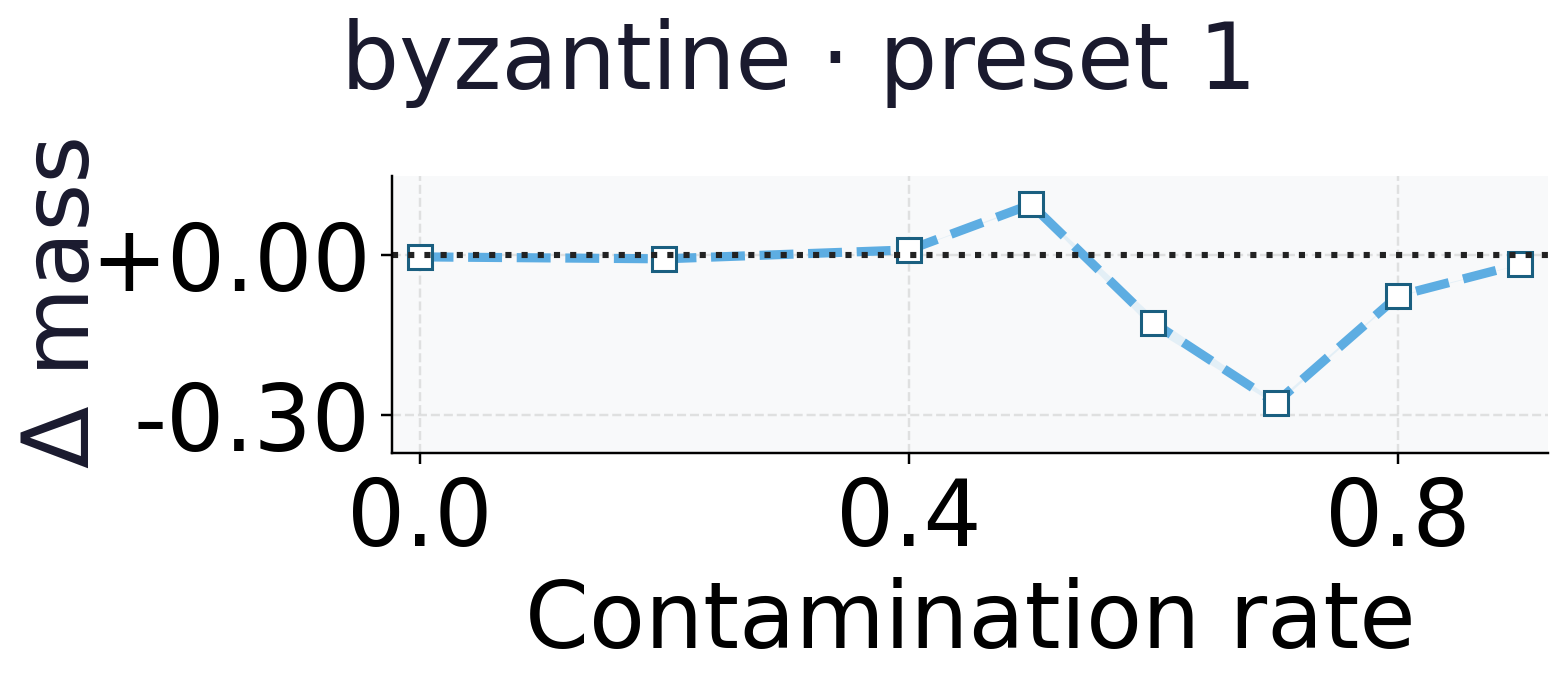
\includegraphics[keepaspectratio,width=0.98\linewidth,height=0.8\textheight,alt={byzantine, preset 1 (RKL): signed mass contrast and its own 95\% seed-bootstrap band; shared mechanism limits.}]{../figures/robustness_review_grid.slide-directional-byzantine-rkl.png}
\refstepcounter{figure}\label{fig:robustness-review-grid-slide-panel-13}
\end{figure}
\end{frame}

\begin{frame}{Selection-free all-method\ldots{} (part 23)}
\begin{figure}
\centering
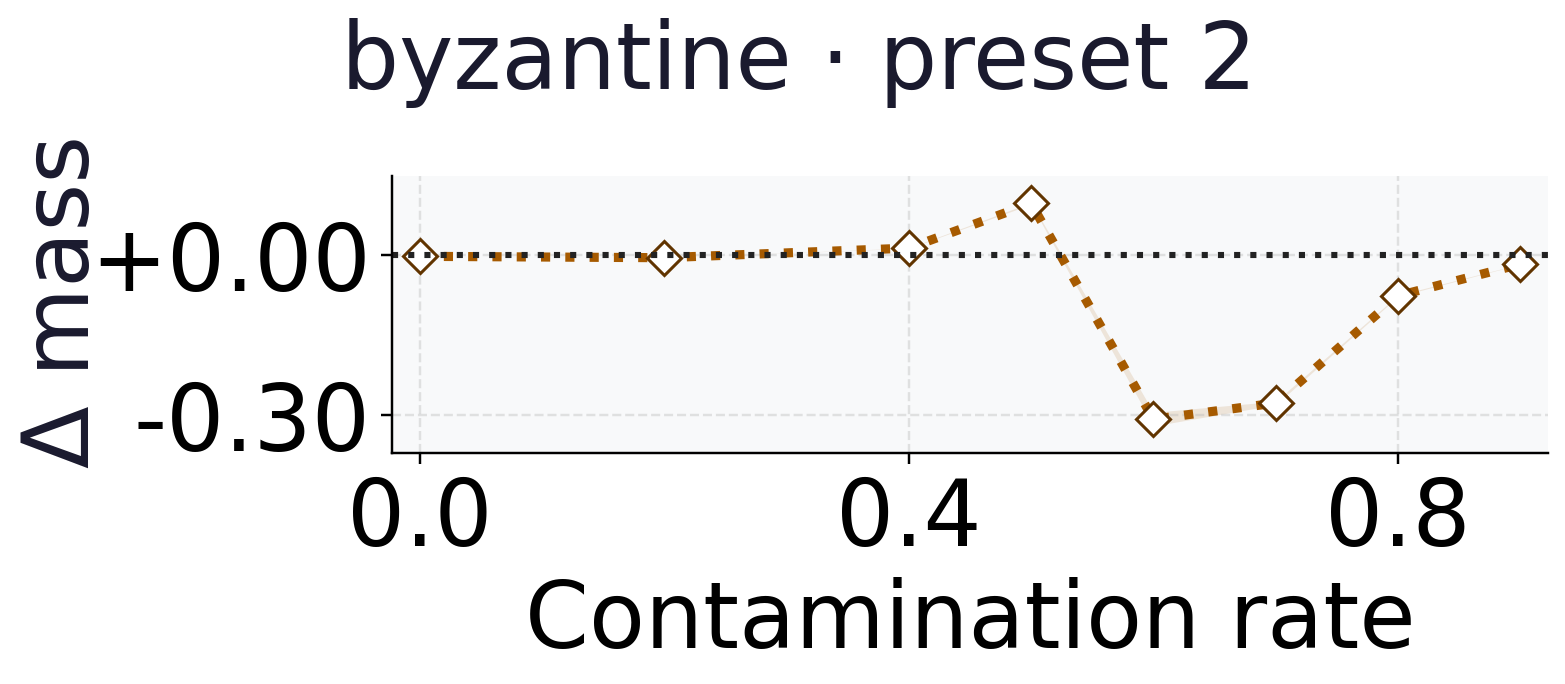
\includegraphics[keepaspectratio,width=0.98\linewidth,height=0.8\textheight,alt={byzantine, preset 2 (AR): signed mass contrast and its own 95\% seed-bootstrap band; shared mechanism limits.}]{../figures/robustness_review_grid.slide-directional-byzantine-ar.png}
\refstepcounter{figure}\label{fig:robustness-review-grid-slide-panel-14}
\end{figure}
\end{frame}

\begin{frame}{Selection-free all-method\ldots{} (part 24)}
\begin{figure}
\centering
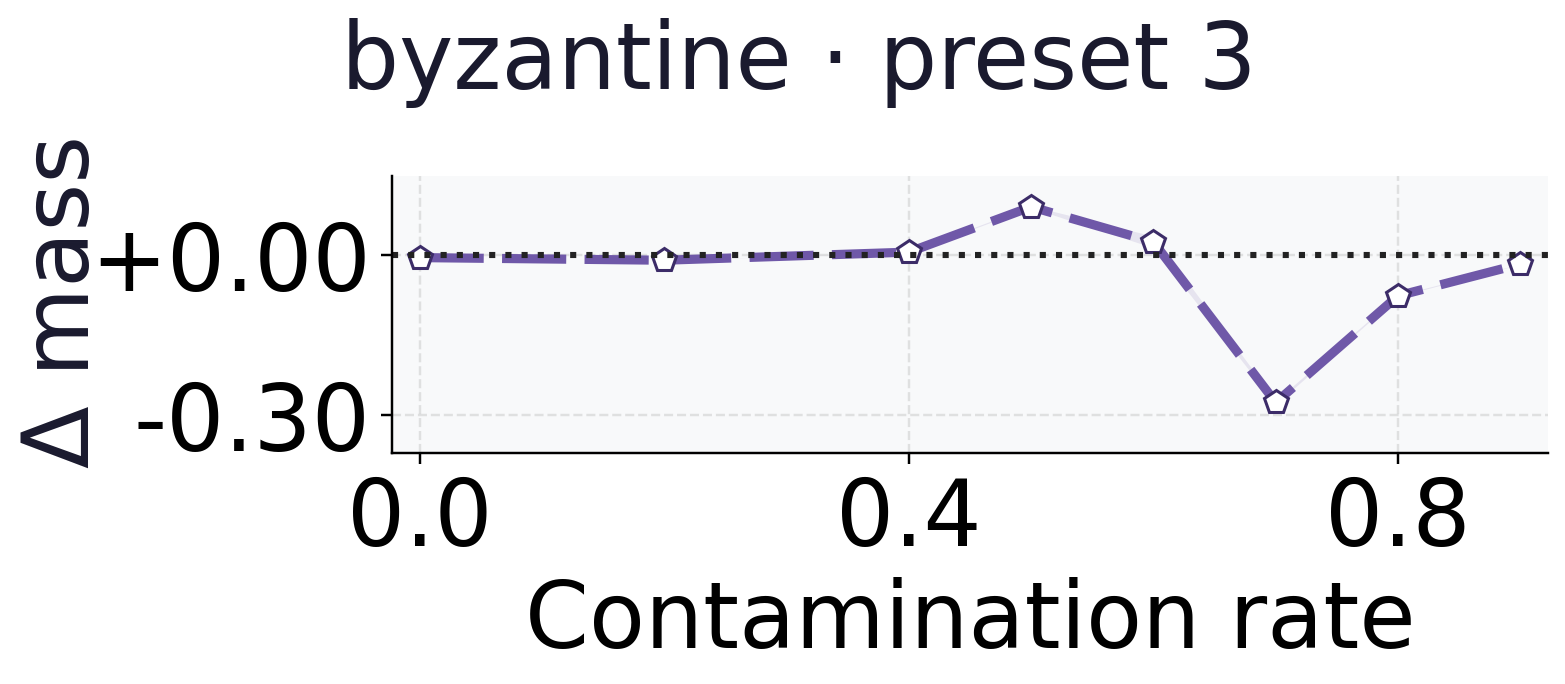
\includegraphics[keepaspectratio,width=0.98\linewidth,height=0.8\textheight,alt={byzantine, preset 3 (beta): signed mass contrast and its own 95\% seed-bootstrap band; shared mechanism limits.}]{../figures/robustness_review_grid.slide-directional-byzantine-beta.png}
\refstepcounter{figure}\label{fig:robustness-review-grid-slide-panel-15}
\end{figure}
\end{frame}

\begin{frame}{Selection-free all-method\ldots{} (part 25)}
\begin{figure}
\centering
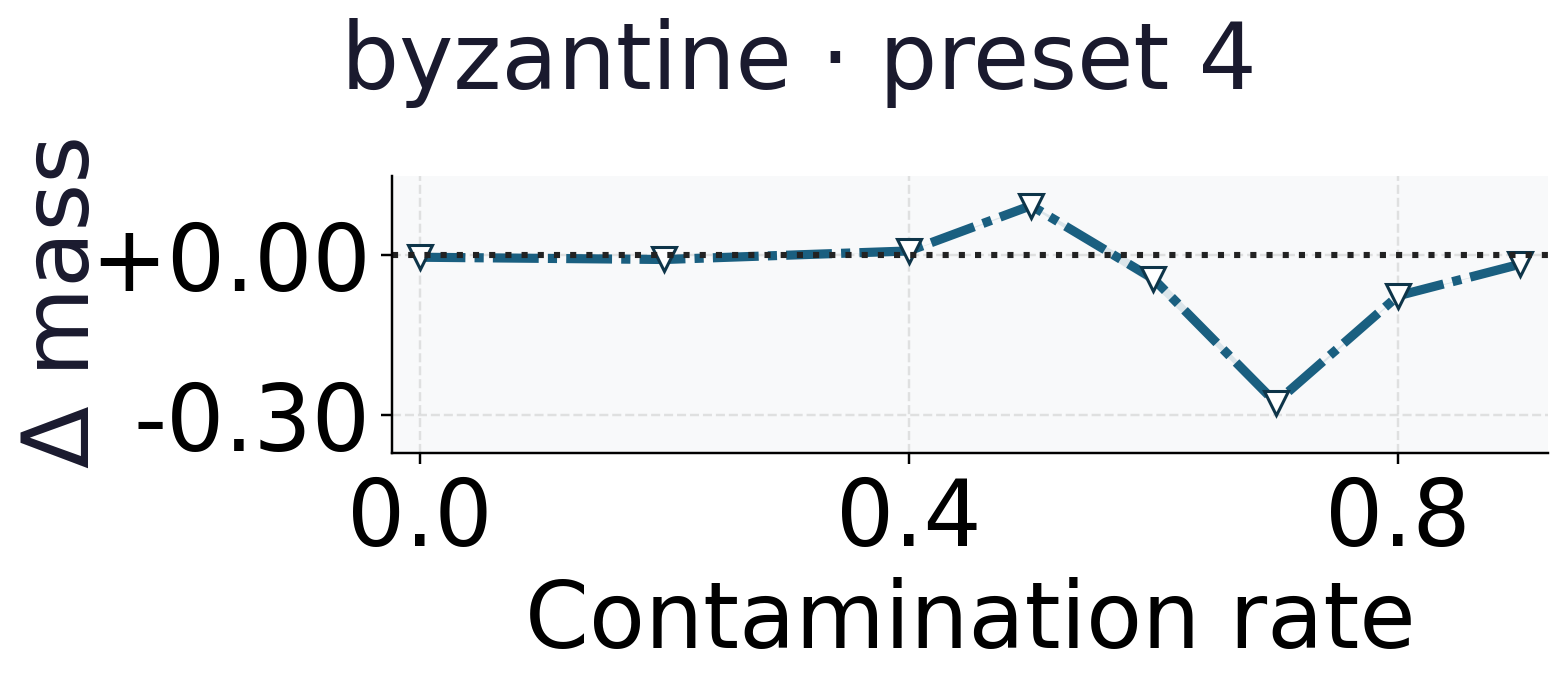
\includegraphics[keepaspectratio,width=0.98\linewidth,height=0.8\textheight,alt={byzantine, preset 4 (rcce): signed mass contrast and its own 95\% seed-bootstrap band; shared mechanism limits.}]{../figures/robustness_review_grid.slide-directional-byzantine-rcce.png}
\refstepcounter{figure}\label{fig:robustness-review-grid-slide-panel-16}
\end{figure}
\end{frame}

\begin{frame}{Selection-free all-method\ldots{} (part 26)}
\begin{figure}
\centering
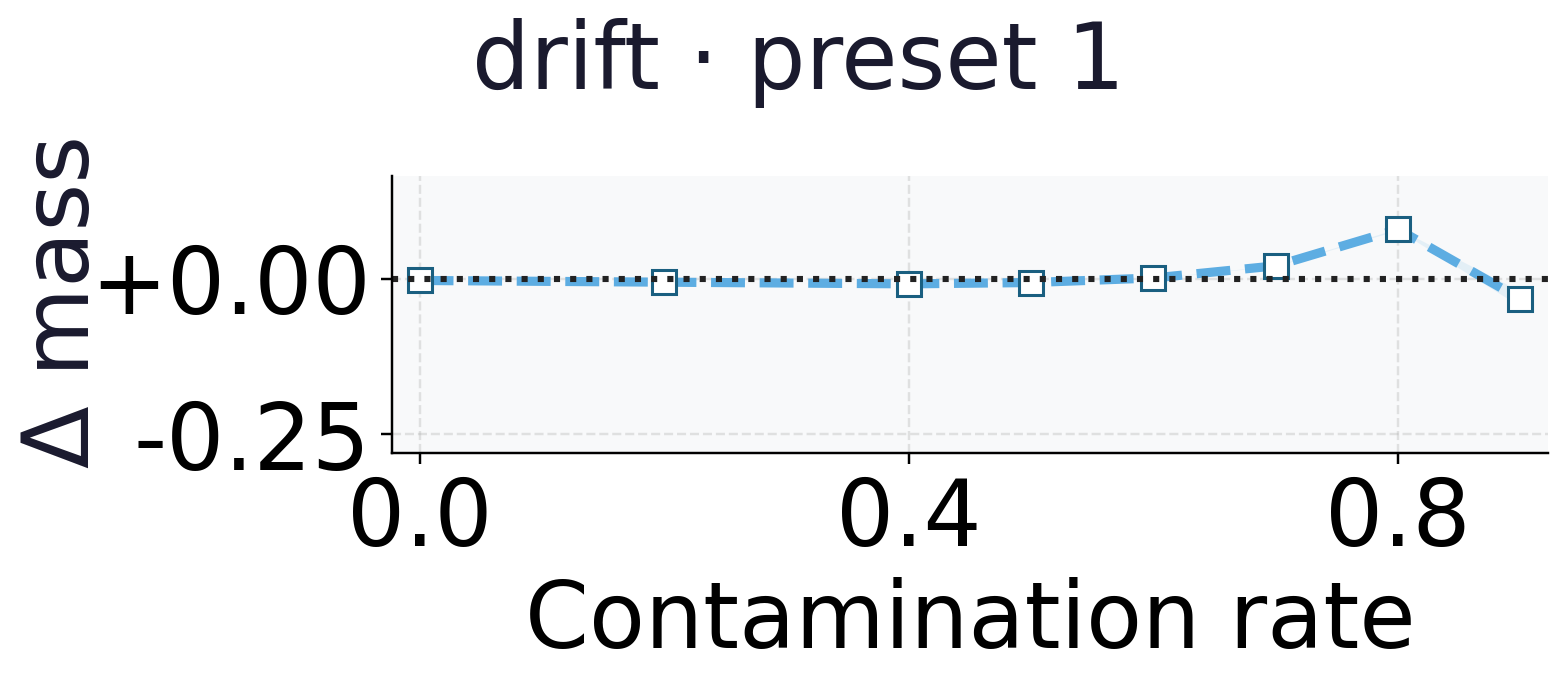
\includegraphics[keepaspectratio,width=0.98\linewidth,height=0.8\textheight,alt={drift, preset 1 (RKL): signed mass contrast and its own 95\% seed-bootstrap band; shared mechanism limits.}]{../figures/robustness_review_grid.slide-directional-drift-rkl.png}
\refstepcounter{figure}\label{fig:robustness-review-grid-slide-panel-17}
\end{figure}
\end{frame}

\begin{frame}{Selection-free all-method\ldots{} (part 27)}
\begin{figure}
\centering
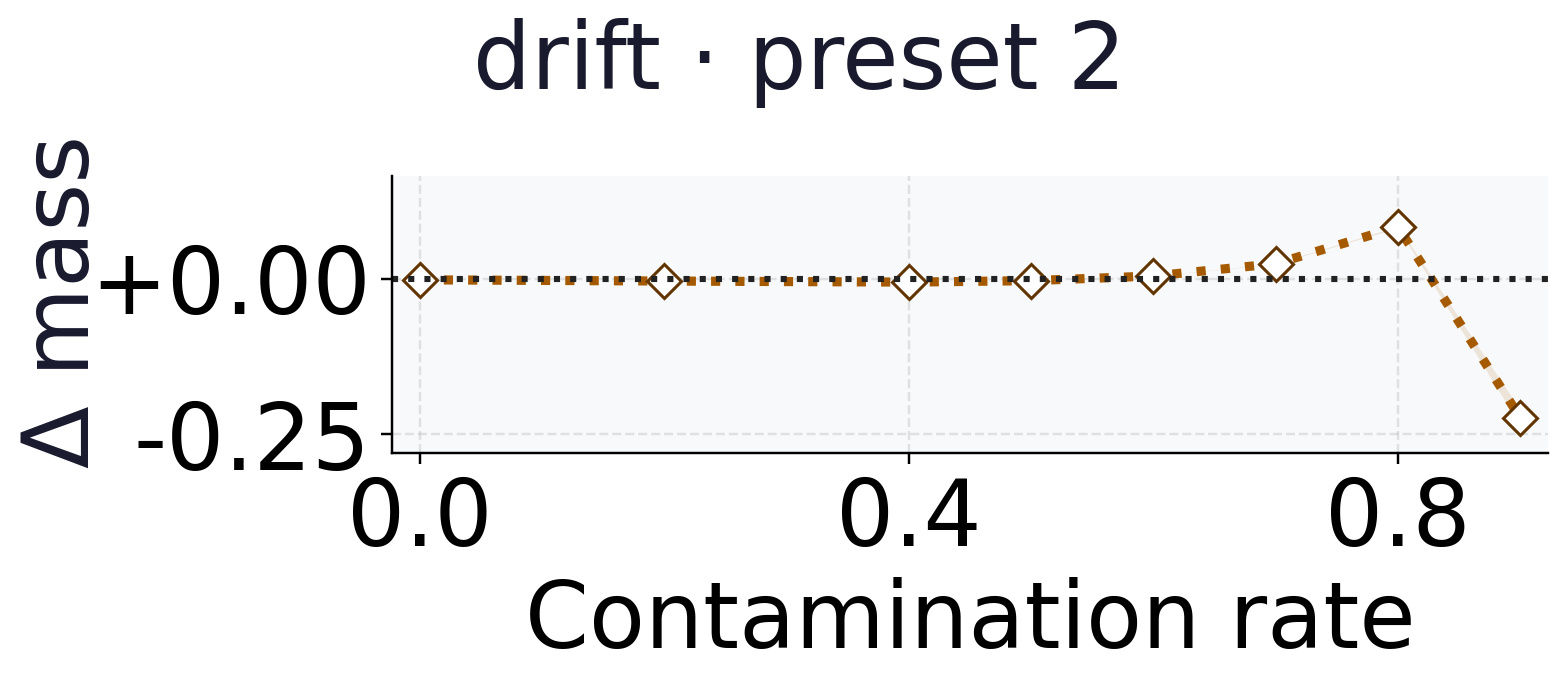
\includegraphics[keepaspectratio,width=0.98\linewidth,height=0.8\textheight,alt={drift, preset 2 (AR): signed mass contrast and its own 95\% seed-bootstrap band; shared mechanism limits.}]{../figures/robustness_review_grid.slide-directional-drift-ar.png}
\refstepcounter{figure}\label{fig:robustness-review-grid-slide-panel-18}
\end{figure}
\end{frame}

\begin{frame}{Selection-free all-method\ldots{} (part 28)}
\begin{figure}
\centering
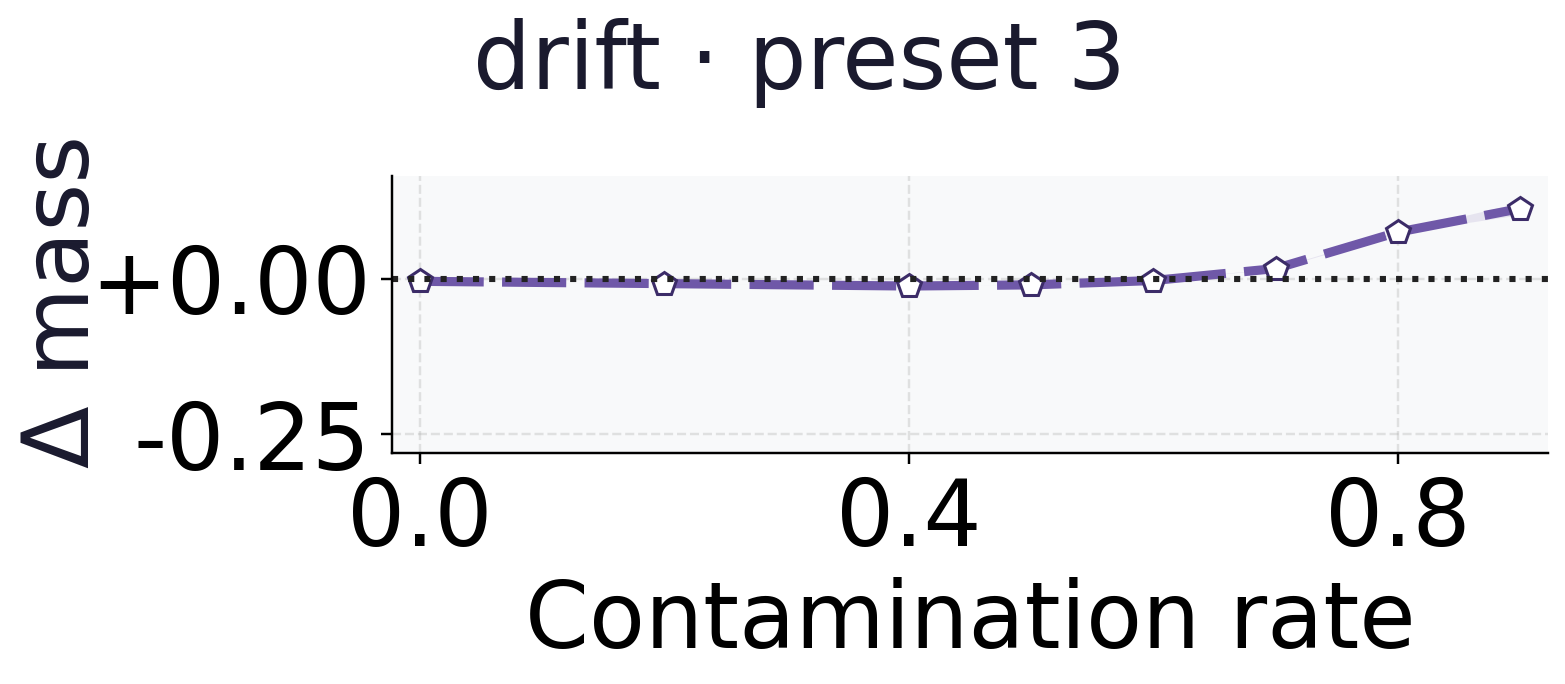
\includegraphics[keepaspectratio,width=0.98\linewidth,height=0.8\textheight,alt={drift, preset 3 (beta): signed mass contrast and its own 95\% seed-bootstrap band; shared mechanism limits.}]{../figures/robustness_review_grid.slide-directional-drift-beta.png}
\refstepcounter{figure}\label{fig:robustness-review-grid-slide-panel-19}
\end{figure}
\end{frame}

\begin{frame}{Selection-free all-method\ldots{} (part 29)}
\begin{figure}
\centering
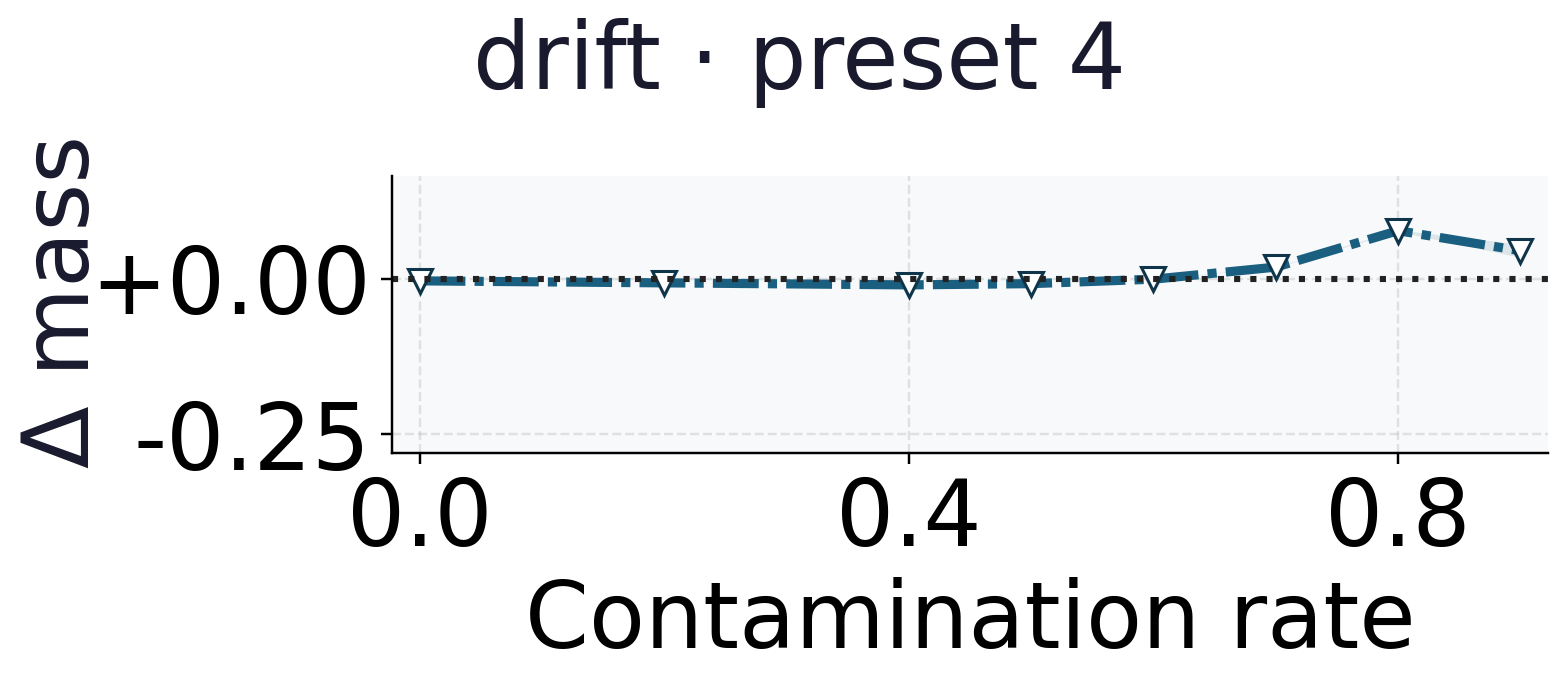
\includegraphics[keepaspectratio,width=0.98\linewidth,height=0.8\textheight,alt={drift, preset 4 (rcce): signed mass contrast and its own 95\% seed-bootstrap band; shared mechanism limits.}]{../figures/robustness_review_grid.slide-directional-drift-rcce.png}
\refstepcounter{figure}\label{fig:robustness-review-grid-slide-panel-20}
\end{figure}
\end{frame}

\begin{frame}{Conditional matched-trial comparison at the declared rate}
\protect\phantomsection\label{sec:results-verdict}
At contamination rate 0.800, each of 960 matched trials redraws the
heterogeneous healthy colony while holding the seeded world's true state
and attack target fixed.
\end{frame}

\begin{frame}{Conditional matched-trial\ldots{} (part 2)}
Each non-reference server preset is compared with the standard pool
using the paired Wilcoxon signed-rank test (Wilcoxon 1945).

Benjamini--Hochberg FDR adjustment applies within the declared family
(Benjamini and Hochberg 1995).
\end{frame}

\begin{frame}[fragile]{Conditional matched-trial\ldots{} (part 3)}
The generated \texttt{Wins} field is true only when the adjusted null is
rejected and the paired effect is positive. It is conditional
bookkeeping for this fixed world and rate, not a universal method
ranking.
\end{frame}

\begin{frame}{Conditional matched-trial\ldots{} (part 4)}
% template-accessible-table-inset
\begingroup
\setlength{\AFSlideTableWidth}{\textwidth}%
\setlength{\LTleft}{\fill}%
\setlength{\LTright}{\fill}%
\begin{longtable}[]{@{}
  >{\raggedright\arraybackslash}p{(\AFSlideTableWidth - 8\tabcolsep) * \real{0.2491}}
  >{\raggedright\arraybackslash}p{(\AFSlideTableWidth - 8\tabcolsep) * \real{0.2242}}
  >{\raggedright\arraybackslash}p{(\AFSlideTableWidth - 8\tabcolsep) * \real{0.1993}}
  >{\raggedright\arraybackslash}p{(\AFSlideTableWidth - 8\tabcolsep) * \real{0.1993}}
  >{\raggedright\arraybackslash}p{(\AFSlideTableWidth - 8\tabcolsep) * \real{0.1282}}@{}}
\label{tbl:robustness_verdict}\tabularnewline
\toprule\noalign{}
\begin{minipage}[b]{\linewidth}\raggedright
Server preset
\end{minipage} & \begin{minipage}[b]{\linewidth}\raggedright
Effect size
\end{minipage} & \begin{minipage}[b]{\linewidth}\raggedright
Raw p
\end{minipage} & \begin{minipage}[b]{\linewidth}\raggedright
q
\end{minipage} & \begin{minipage}[b]{\linewidth}\raggedright
Wins
\end{minipage} \\
\midrule\noalign{}
\endfirsthead
\toprule\noalign{}
\begin{minipage}[b]{\linewidth}\raggedright
Server preset
\end{minipage} & \begin{minipage}[b]{\linewidth}\raggedright
Effect size
\end{minipage} & \begin{minipage}[b]{\linewidth}\raggedright
Raw p
\end{minipage} & \begin{minipage}[b]{\linewidth}\raggedright
q
\end{minipage} & \begin{minipage}[b]{\linewidth}\raggedright
Wins
\end{minipage} \\
\midrule\noalign{}
\endhead
AR & 1.0000 & 1.11e-158 & 1.11e-158 & Yes \\
RKL & 1.0000 & 1.11e-158 & 1.11e-158 & Yes \\
beta & 1.0000 & 1.11e-158 & 1.11e-158 & Yes \\
rcce & 1.0000 & 1.11e-158 & 1.11e-158 & Yes \\
\bottomrule\noalign{}
\end{longtable}
\endgroup
\end{frame}

\begin{frame}{Conditional matched-trial\ldots{} (part 5)}
% template-accessible-table-inset
\begingroup
\setlength{\AFSlideTableWidth}{\textwidth}%
\setlength{\LTleft}{\fill}%
\setlength{\LTright}{\fill}%
\begin{longtable}[]{@{}
  >{\raggedright\arraybackslash}p{(\AFSlideTableWidth - 8\tabcolsep) * \real{0.1795}}
  >{\raggedright\arraybackslash}p{(\AFSlideTableWidth - 8\tabcolsep) * \real{0.2308}}
  >{\raggedright\arraybackslash}p{(\AFSlideTableWidth - 8\tabcolsep) * \real{0.1282}}
  >{\raggedright\arraybackslash}p{(\AFSlideTableWidth - 8\tabcolsep) * \real{0.2517}}
  >{\raggedright\arraybackslash}p{(\AFSlideTableWidth - 8\tabcolsep) * \real{0.2098}}@{}}
\label{tbl:verdict-effect-estimates}\tabularnewline
\toprule\noalign{}
\begin{minipage}[b]{\linewidth}\raggedright
Method
\end{minipage} & \begin{minipage}[b]{\linewidth}\raggedright
Derived \(d_{\rm eq}\)
\end{minipage} & \begin{minipage}[b]{\linewidth}\raggedright
Label
\end{minipage} & \begin{minipage}[b]{\linewidth}\raggedright
Mean \(\Delta\) accuracy
\end{minipage} & \begin{minipage}[b]{\linewidth}\raggedright
95\% CI
\end{minipage} \\
\midrule\noalign{}
\endfirsthead
\toprule\noalign{}
\begin{minipage}[b]{\linewidth}\raggedright
Method
\end{minipage} & \begin{minipage}[b]{\linewidth}\raggedright
Derived \(d_{\rm eq}\)
\end{minipage} & \begin{minipage}[b]{\linewidth}\raggedright
Label
\end{minipage} & \begin{minipage}[b]{\linewidth}\raggedright
Mean \(\Delta\) accuracy
\end{minipage} & \begin{minipage}[b]{\linewidth}\raggedright
95\% CI
\end{minipage} \\
\midrule\noalign{}
\endhead
AR & saturated (r=+1) & large & 0.0846 & {[}0.0821, 0.0873{]} \\
RKL & saturated (r=+1) & large & 0.0809 & {[}0.0783, 0.0834{]} \\
\bottomrule\noalign{}
\end{longtable}
\endgroup
\end{frame}

\begin{frame}{Conditional matched-trial\ldots{} (part 6)}
% template-accessible-table-inset
\begingroup
\setlength{\AFSlideTableWidth}{\textwidth}%
\setlength{\LTleft}{\fill}%
\setlength{\LTright}{\fill}%
\begin{longtable}[]{@{}
  >{\raggedright\arraybackslash}p{(\AFSlideTableWidth - 10\tabcolsep) * \real{0.1842}}
  >{\raggedright\arraybackslash}p{(\AFSlideTableWidth - 10\tabcolsep) * \real{0.1429}}
  >{\raggedright\arraybackslash}p{(\AFSlideTableWidth - 10\tabcolsep) * \real{0.1429}}
  >{\raggedright\arraybackslash}p{(\AFSlideTableWidth - 10\tabcolsep) * \real{0.1579}}
  >{\raggedright\arraybackslash}p{(\AFSlideTableWidth - 10\tabcolsep) * \real{0.2143}}
  >{\raggedright\arraybackslash}p{(\AFSlideTableWidth - 10\tabcolsep) * \real{0.1579}}@{}}
\label{tbl:verdict-inference-power}\tabularnewline
\toprule\noalign{}
\begin{minipage}[b]{\linewidth}\raggedright
Method
\end{minipage} & \begin{minipage}[b]{\linewidth}\raggedright
Raw p
\end{minipage} & \begin{minipage}[b]{\linewidth}\raggedright
q
\end{minipage} & \begin{minipage}[b]{\linewidth}\raggedright
Power
\end{minipage} & \begin{minipage}[b]{\linewidth}\raggedright
Target \(n_{\rm trial}\)
\end{minipage} & \begin{minipage}[b]{\linewidth}\raggedright
Reject
\end{minipage} \\
\midrule\noalign{}
\endfirsthead
\toprule\noalign{}
\begin{minipage}[b]{\linewidth}\raggedright
Method
\end{minipage} & \begin{minipage}[b]{\linewidth}\raggedright
Raw p
\end{minipage} & \begin{minipage}[b]{\linewidth}\raggedright
q
\end{minipage} & \begin{minipage}[b]{\linewidth}\raggedright
Power
\end{minipage} & \begin{minipage}[b]{\linewidth}\raggedright
Target \(n_{\rm trial}\)
\end{minipage} & \begin{minipage}[b]{\linewidth}\raggedright
Reject
\end{minipage} \\
\midrule\noalign{}
\endhead
AR & 1.11e-158 & 1.11e-158 & 1.0000 & 5 & Yes \\
RKL & 1.11e-158 & 1.11e-158 & 1.0000 & 5 & Yes \\
\bottomrule\noalign{}
\end{longtable}
\endgroup
\end{frame}

\begin{frame}{Conditional matched-trial\ldots{} (part 7)}
% template-accessible-table-inset
\begingroup
\setlength{\AFSlideTableWidth}{\textwidth}%
\setlength{\LTleft}{\fill}%
\setlength{\LTright}{\fill}%
\begin{longtable}[]{@{}
  >{\raggedright\arraybackslash}p{(\AFSlideTableWidth - 6\tabcolsep) * \real{0.2000}}
  >{\raggedright\arraybackslash}p{(\AFSlideTableWidth - 6\tabcolsep) * \real{0.1429}}
  >{\raggedright\arraybackslash}p{(\AFSlideTableWidth - 6\tabcolsep) * \real{0.3714}}
  >{\raggedright\arraybackslash}p{(\AFSlideTableWidth - 6\tabcolsep) * \real{0.2857}}@{}}
\label{tbl:accuracy-at-verdict}\tabularnewline
\toprule\noalign{}
\begin{minipage}[b]{\linewidth}\raggedright
Method
\end{minipage} & \begin{minipage}[b]{\linewidth}\raggedright
n
\end{minipage} & \begin{minipage}[b]{\linewidth}\raggedright
Mean acc. @ verdict rate
\end{minipage} & \begin{minipage}[b]{\linewidth}\raggedright
95\% CI
\end{minipage} \\
\midrule\noalign{}
\endfirsthead
\toprule\noalign{}
\begin{minipage}[b]{\linewidth}\raggedright
Method
\end{minipage} & \begin{minipage}[b]{\linewidth}\raggedright
n
\end{minipage} & \begin{minipage}[b]{\linewidth}\raggedright
Mean acc. @ verdict rate
\end{minipage} & \begin{minipage}[b]{\linewidth}\raggedright
95\% CI
\end{minipage} \\
\midrule\noalign{}
\endhead
KLD & 960 & 0.9021 & {[}0.8993, 0.9049{]} \\
RKL & 960 & 0.9829 & {[}0.9827, 0.9832{]} \\
\bottomrule\noalign{}
\end{longtable}
\endgroup
\end{frame}

\begin{frame}{Conditional matched-trial\ldots{} (part 8)}
\textbf{Reference mean.} Naive-pool mean accuracy at the verdict rate is
0.9021 (per-trial mean over 960 trials; the bootstrap CI is in
tbl.~10).

\textbf{Positive contrasts.} At least one non-reference preset is a
BH-rejected positive contrast: Yes.
\end{frame}

\begin{frame}{Conditional matched-trial\ldots{} (part 9)}
\textbf{Headline display.} The method is RKL (tied set: RKL, AR, beta,
rcce), with rank-biserial-derived \(d\)-equivalent saturated (r=+1)
(large), mean accuracy difference 0.0809 (\([0.0783, 0.0834]\)), raw
\(p = 1.11 \times 10^{-158}\), and \(q = 1.11 \times 10^{-158}\).
\end{frame}

\begin{frame}{Conditional matched-trial\ldots{} (part 10)}
Its observed-effect design power is 1.0000. Prospective \(n\) for power
0.80 is 5.
\end{frame}

\begin{frame}{Conditional matched-trial\ldots{} (part 11)}
\textbf{Display rule.} Under largest positive rank-biserial
effect\_size; stable method order tie-break (tie-break: first robust
method in divergences order), observed-effect design power is 1.0000 at
the run's \(n_{\rm trial} = 960\).
\end{frame}

\begin{frame}{Conditional matched-trial\ldots{} (part 12)}
A confirmatory replication should budget \(n_{\rm trial} = 5\) for power
0.80 (prospective \(n = 7\)).
\end{frame}

\begin{frame}{Conditional matched-trial\ldots{} (part 13)}
The standard pool degrades and some non-reference presets have positive
conditional contrasts. The statistics module produces the paired tests,
multiple-testing adjustment, bootstrap intervals, and planning analysis;
the prose does not promote them beyond their matched-trial estimand.
\end{frame}

\begin{frame}{Conditional matched-trial\ldots{} (part 14)}
The headline label is a deterministic display choice, not a unique
scientific winner. The complete tied set is RKL, AR, beta, rcce, the
largest paired mean-difference method is AR, and the worst-rate pooled
display method is beta. These may differ because they answer different
descriptive questions.
\end{frame}

\begin{frame}[fragile]{Server-side heuristic axis: conditional contrasts
without theorem transfer}
\protect\phantomsection\label{server-side-heuristic-axis-conditional-contrasts-without-theorem-transfer}
The comparison above belongs to the heuristic server axis defined in
sec.~3.3. fig.~15 visualizes
the \texttt{robust\_aggregate} divergence-reweighting that down-weights
agents at pooling time.
\end{frame}

\begin{frame}{Server-side heuristic axis (part 2)}
Its positive formal property is the naive-recovery limit of Theorem
5 (eq.~10, the 0
residual of sec.~7.1),
\end{frame}

\begin{frame}{Server-side heuristic axis (part 3)}
and it has a scoped no-go result for a declared separable objective
class, not an objective certificate.
\end{frame}

\begin{frame}{Server-side heuristic axis (part 4)}
The heuristic carries no bounded-influence guarantee. The effect sizes,
intervals, and planning quantities characterize its conditional
contrasts; they do not certify the per-agent generalized-Bayes claim,
which remains separately source-conditional in
sec.~7.6.
\end{frame}

\begin{frame}{Server-side heuristic axis (part 5)}
\begin{figure}
\centering
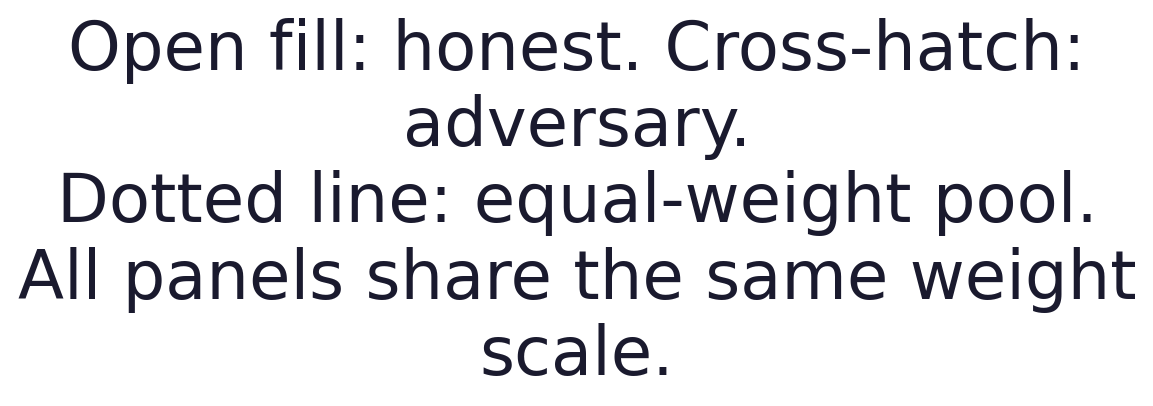
\includegraphics[keepaspectratio,width=0.98\linewidth,height=0.8\textheight,alt={Open fill: honest. Cross-hatch: adversary.
Dotted line: equal-weight pool.
All panels share the same weight scale.}]{../figures/robust_influence_weights.slide-encoding.png}
\refstepcounter{figure}\label{fig:robust-weights-slide-panel-1}
\end{figure}
\end{frame}

\begin{frame}{Server-side heuristic axis (part 6)}
\begin{figure}
\centering
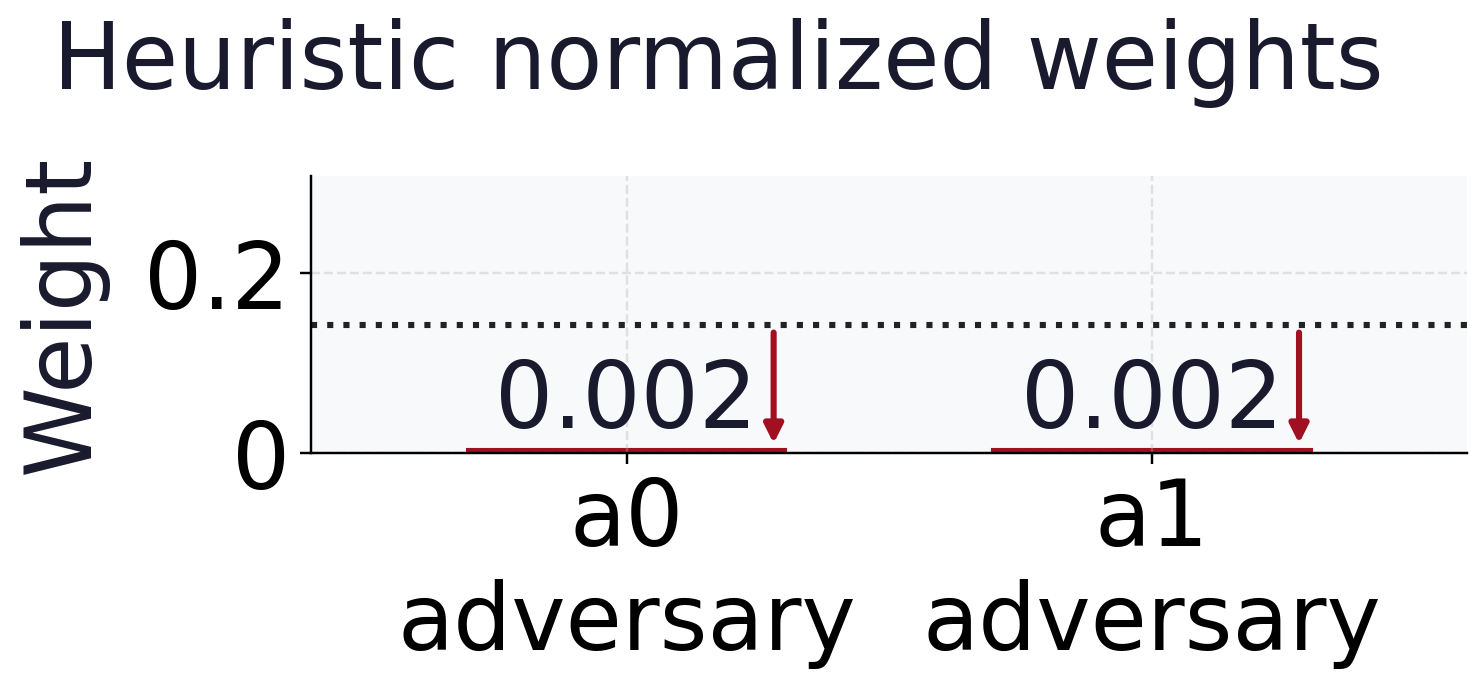
\includegraphics[keepaspectratio,width=0.98\linewidth,height=0.8\textheight,alt={Agents 0 through 1: exact normalized heuristic weights; shared scale and equal-weight reference.}]{../figures/robust_influence_weights.slide-agents-1-2.png}
\refstepcounter{figure}\label{fig:robust-weights-slide-panel-2}
\end{figure}
\end{frame}

\begin{frame}{Server-side heuristic axis (part 7)}
\begin{figure}
\centering
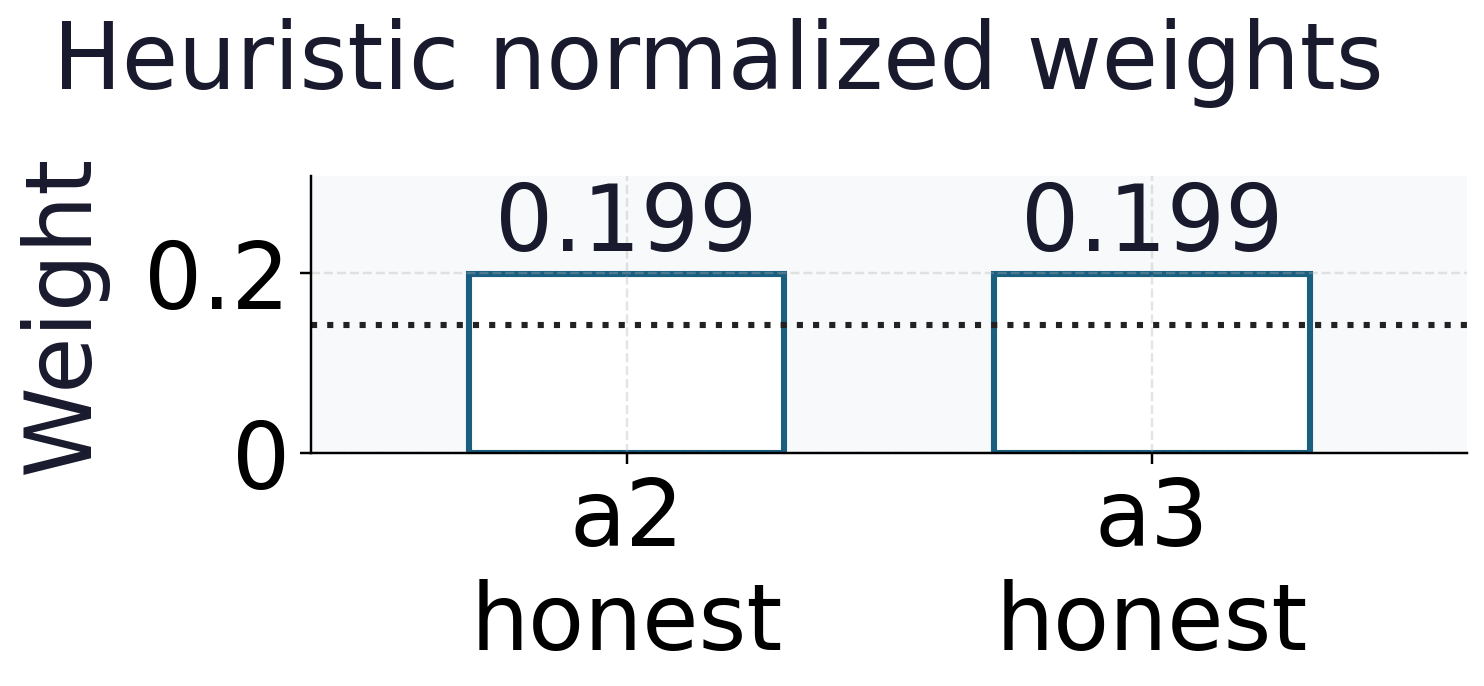
\includegraphics[keepaspectratio,width=0.98\linewidth,height=0.8\textheight,alt={Agents 2 through 3: exact normalized heuristic weights; shared scale and equal-weight reference.}]{../figures/robust_influence_weights.slide-agents-3-4.png}
\refstepcounter{figure}\label{fig:robust-weights-slide-panel-3}
\end{figure}
\end{frame}

\begin{frame}{Server-side heuristic axis (part 8)}
\begin{figure}
\centering
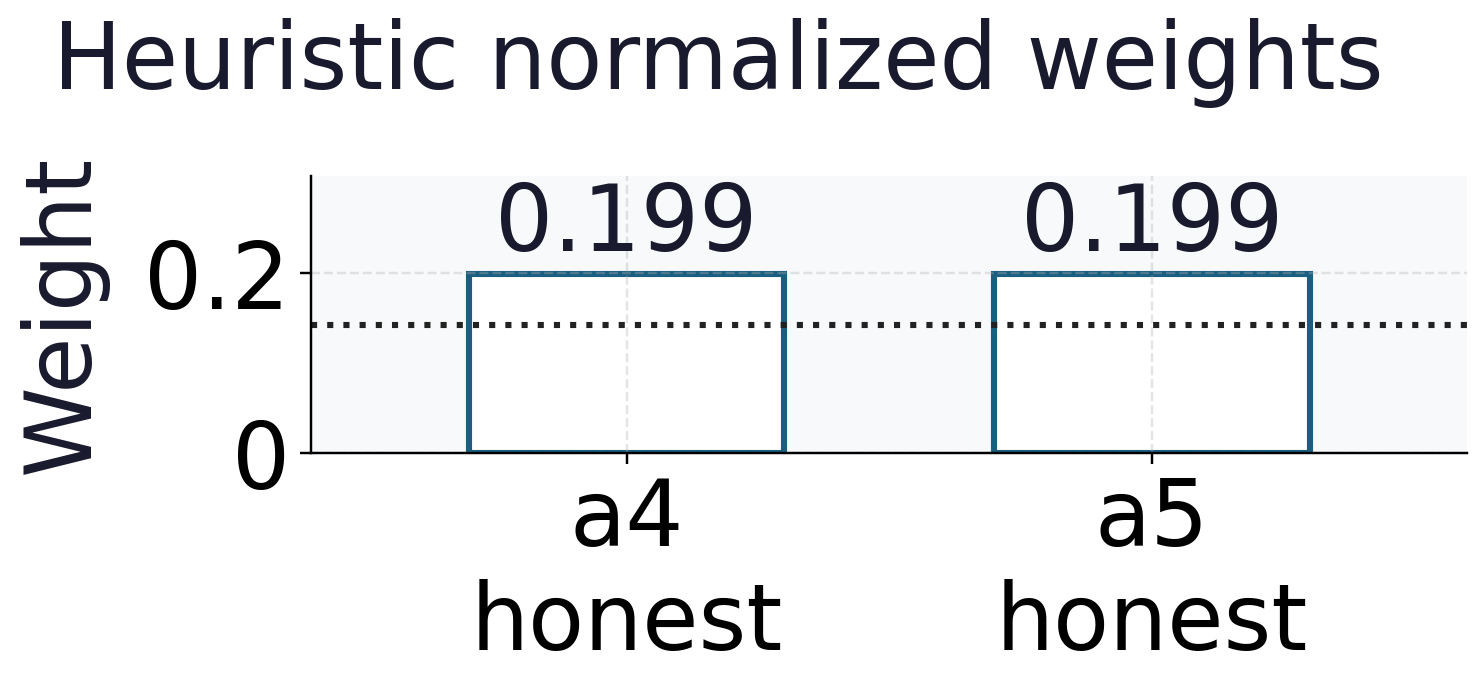
\includegraphics[keepaspectratio,width=0.98\linewidth,height=0.8\textheight,alt={Agents 4 through 5: exact normalized heuristic weights; shared scale and equal-weight reference.}]{../figures/robust_influence_weights.slide-agents-5-6.png}
\refstepcounter{figure}\label{fig:robust-weights-slide-panel-4}
\end{figure}
\end{frame}

\begin{frame}{Server-side heuristic axis (part 9)}
\begin{figure}
\centering
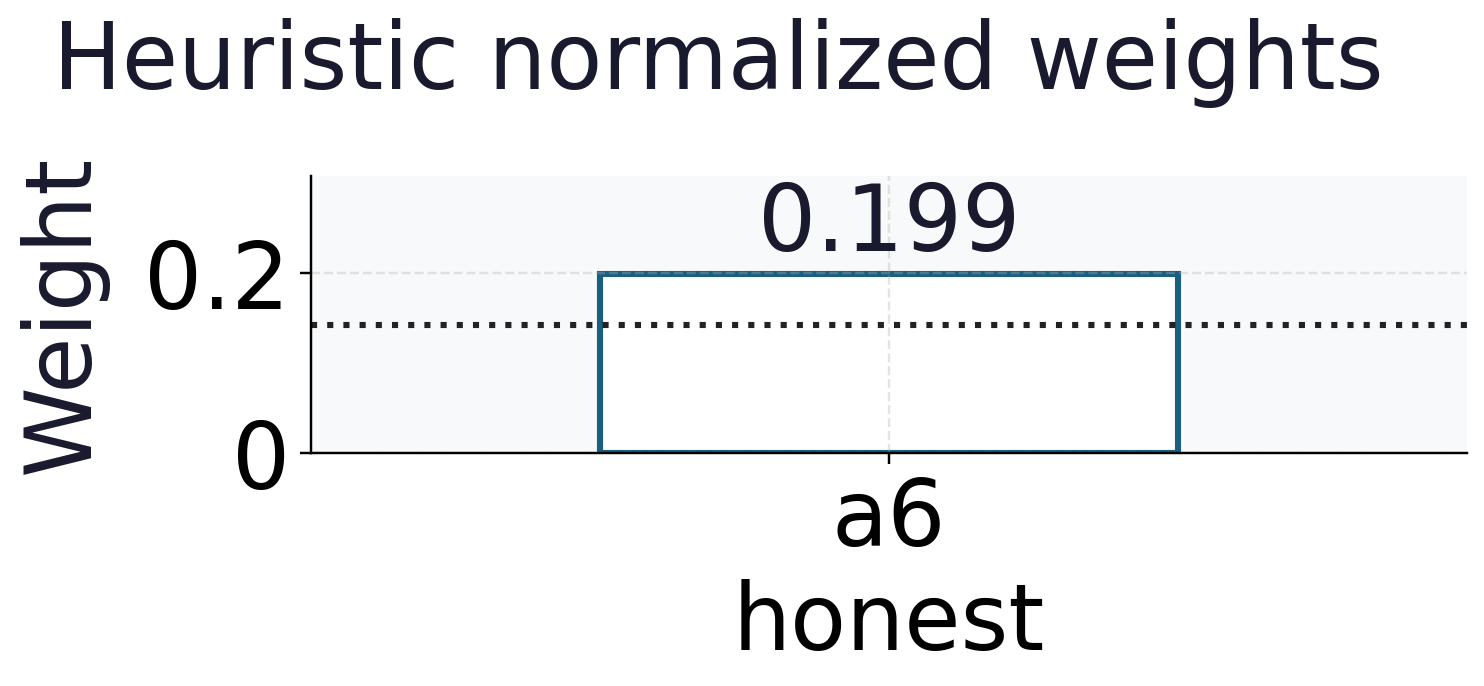
\includegraphics[keepaspectratio,width=0.98\linewidth,height=0.8\textheight,alt={Agents 6 through 6: exact normalized heuristic weights; shared scale and equal-weight reference.}]{../figures/robust_influence_weights.slide-agents-7-7.png}
\refstepcounter{figure}\label{fig:robust-weights-slide-panel-5}
\end{figure}
\end{frame}

\begin{frame}{Server-side heuristic axis (part 10)}
\begin{figure}
\centering
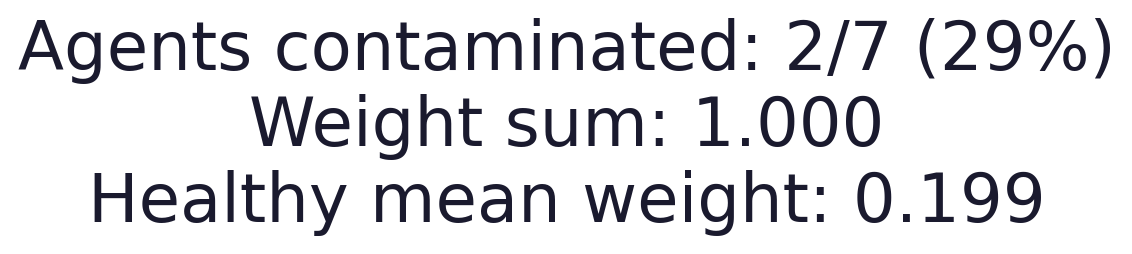
\includegraphics[keepaspectratio,width=0.98\linewidth,height=0.8\textheight,alt={Agents contaminated: 2/7 (29\%)
Weight sum: 1.000
Healthy mean weight: 0.199}]{../figures/robust_influence_weights.slide-notes-1.png}
\refstepcounter{figure}\label{fig:robust-weights-slide-panel-6}
\end{figure}
\end{frame}

\begin{frame}{Server-side heuristic axis (part 11)}
\begin{figure}
\centering
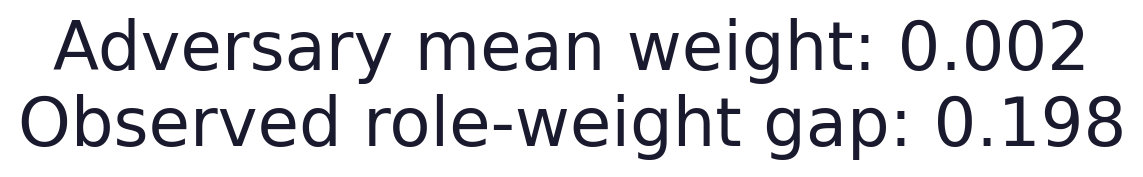
\includegraphics[keepaspectratio,width=0.98\linewidth,height=0.8\textheight,alt={Adversary mean weight: 0.002
Observed role-weight gap: 0.198}]{../figures/robust_influence_weights.slide-notes-2.png}
\refstepcounter{figure}\label{fig:robust-weights-slide-panel-7}
\end{figure}
\end{frame}

\begin{frame}{Server-side heuristic axis (part 12)}
\begin{figure}
\centering
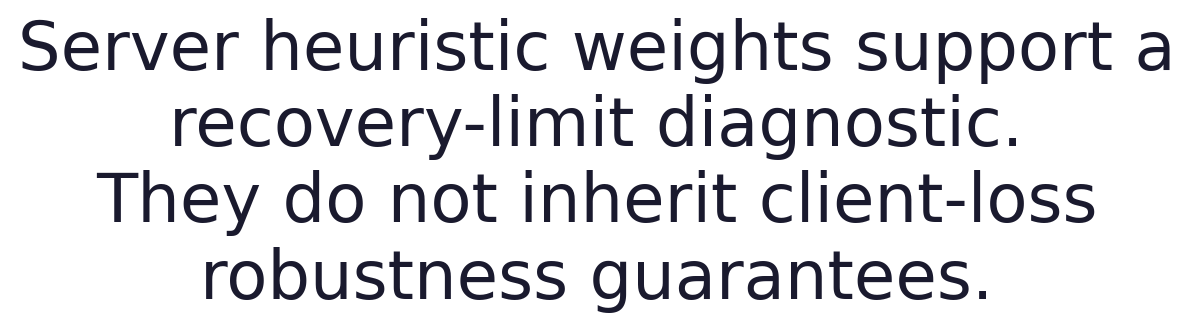
\includegraphics[keepaspectratio,width=0.98\linewidth,height=0.8\textheight,alt={Server heuristic weights support a recovery-limit diagnostic.
They do not inherit client-loss robustness guarantees.}]{../figures/robust_influence_weights.slide-scope.png}
\refstepcounter{figure}\label{fig:robust-weights-slide-panel-8}
\end{figure}
\end{frame}

\begin{frame}{Variational aggregator: conservative objective-backed
weight control}
\protect\phantomsection\label{sec:results-variational}
The heuristic has the higher point accuracy in the configured verdict
cell. The variational aggregator of sec.~5.8.2,
derived in sec.~12, is its objective-backed
complement.
\end{frame}

\begin{frame}{Variational aggregator (part 2)}
Each exact block update does not increase the stated free energy
eq.~12, and a converged fixed point is
coordinatewise stationary. Two deterministic runs show its weight
behavior at robustness 1.50.
\end{frame}

\begin{frame}{Variational aggregator (part 3)}
First, the descent. On a contaminated colony the free energy falls
monotonically from 3.2458 to 2.3780 (a drop of 0.8678 over 11
block-coordinate iterations, converged: Yes), with a largest single-step
\emph{increase} of 8.88e-16 --- machine zero, the numerical witness of
the descent theorem (sec.~12.3).
\end{frame}

\begin{frame}{Variational aggregator (part 4)}
\begin{figure}
\centering
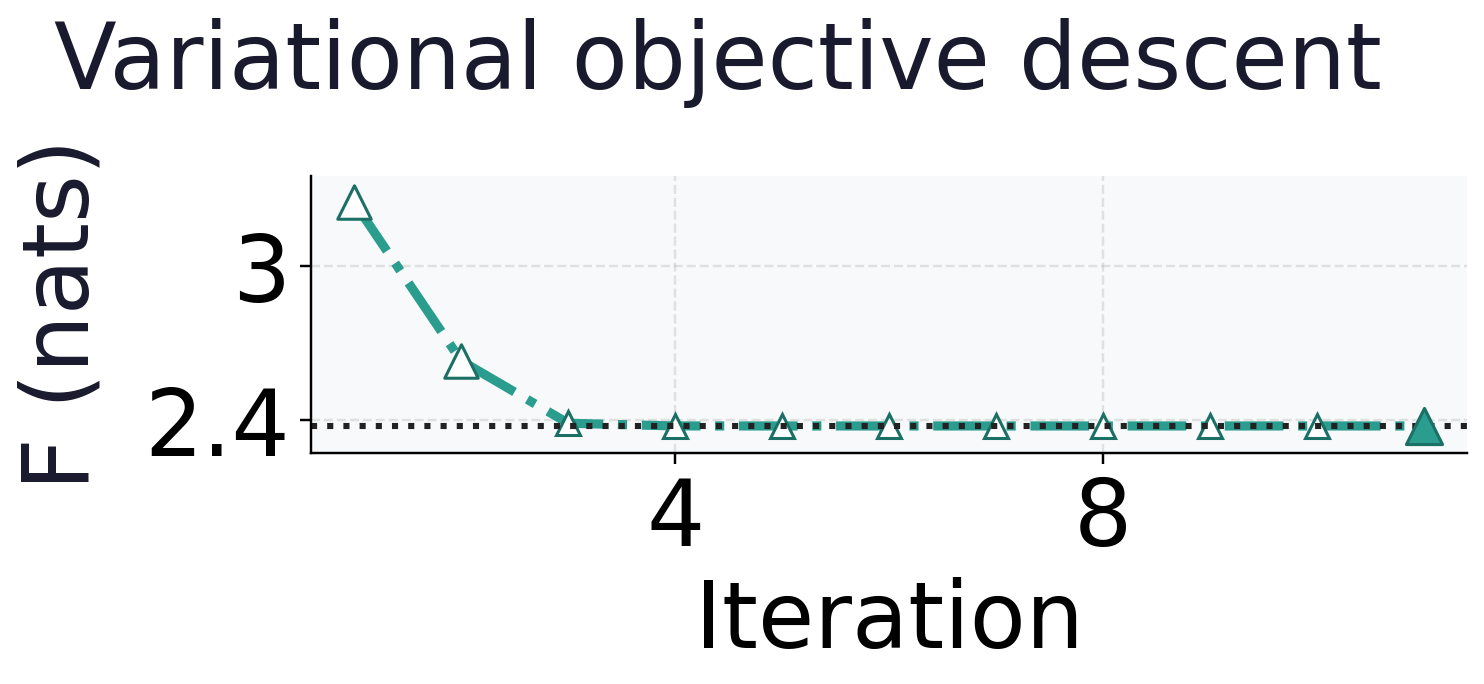
\includegraphics[keepaspectratio,width=0.98\linewidth,height=0.8\textheight,alt={Variational objective in nats at every iteration; filled triangle is final iterate, large open triangles mark the largest observed step.}]{../figures/aggregation_descent.slide-trajectory.png}
\refstepcounter{figure}\label{fig:aggregation-descent-slide-panel-1}
\end{figure}
\end{frame}

\begin{frame}{Variational aggregator (part 5)}
\begin{figure}
\centering
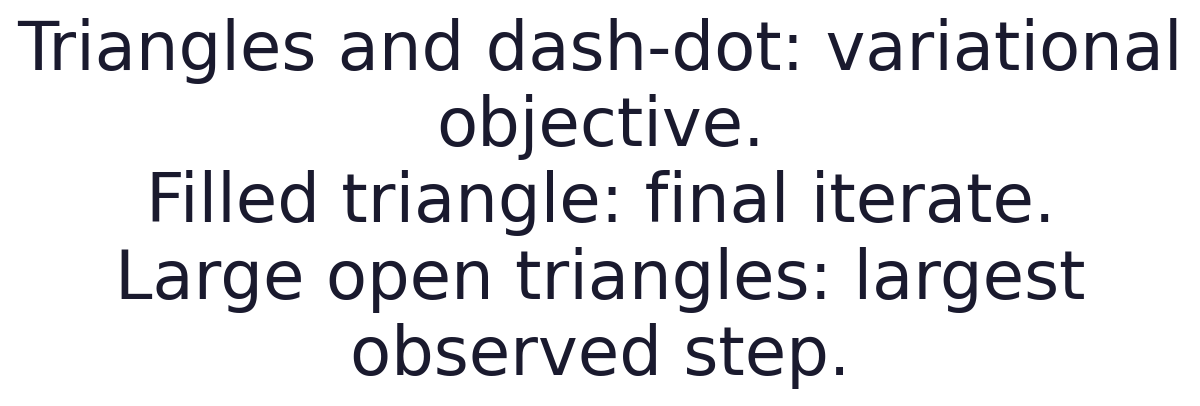
\includegraphics[keepaspectratio,width=0.98\linewidth,height=0.8\textheight,alt={Triangles and dash-dot: variational objective.
Filled triangle: final iterate.
Large open triangles: largest observed step.}]{../figures/aggregation_descent.slide-encoding.png}
\refstepcounter{figure}\label{fig:aggregation-descent-slide-panel-2}
\end{figure}
\end{frame}

\begin{frame}{Variational aggregator (part 6)}
\begin{figure}
\centering

\includegraphics[keepaspectratio,width=0.98\linewidth,height=0.8\textheight,alt={Iterations: 11
Total drop ΔF = 0.868 nats
Max ascent step = 8.9e-16 nats}]{../figures/aggregation_descent.slide-notes-1.png}
\refstepcounter{figure}\label{fig:aggregation-descent-slide-panel-3}
\end{figure}
\end{frame}

\begin{frame}{Variational aggregator (part 7)}
\begin{figure}
\centering

\includegraphics[keepaspectratio,width=0.98\linewidth,height=0.8\textheight,alt={Monotone: yes  ✓ converged}]{../figures/aggregation_descent.slide-notes-2.png}
\refstepcounter{figure}\label{fig:aggregation-descent-slide-panel-4}
\end{figure}
\end{frame}

\begin{frame}{Variational aggregator (part 8)}
\begin{figure}
\centering
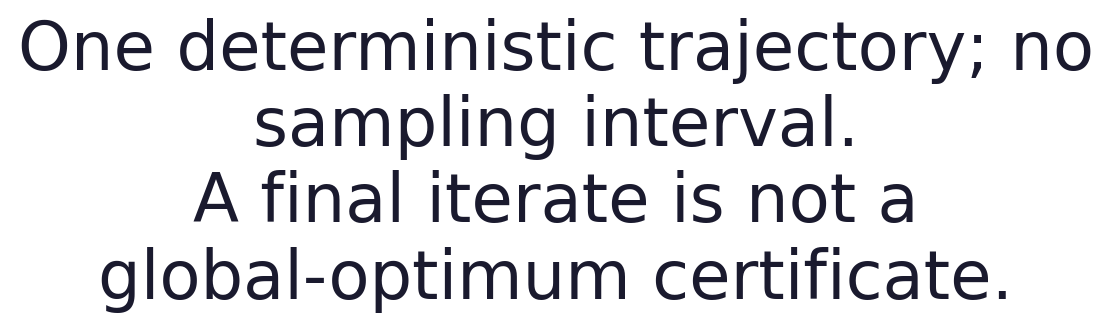
\includegraphics[keepaspectratio,width=0.98\linewidth,height=0.8\textheight,alt={One deterministic trajectory; no sampling interval.
A final iterate is not a global-optimum certificate.}]{../figures/aggregation_descent.slide-scope.png}
\refstepcounter{figure}\label{fig:aggregation-descent-slide-panel-5}
\end{figure}
\end{frame}

\begin{frame}{Variational aggregator (part 9)}
Second, the effective-weight response. As one agent is drifted from
healthy toward a confident-wrong delta, its normalized influence falls
from 0.143 to below 0.001 --- a factor of 267.1 below the fixed 0.143
the naive log-linear pool grants every agent regardless of how wrong it
is.
\end{frame}

\begin{frame}{Variational aggregator (part 10)}
The gap between the falling variational curve and the flat naive line is
the empirical redescending weight response, drawn.
\end{frame}

\begin{frame}{Variational aggregator (part 11)}
\begin{figure}
\centering
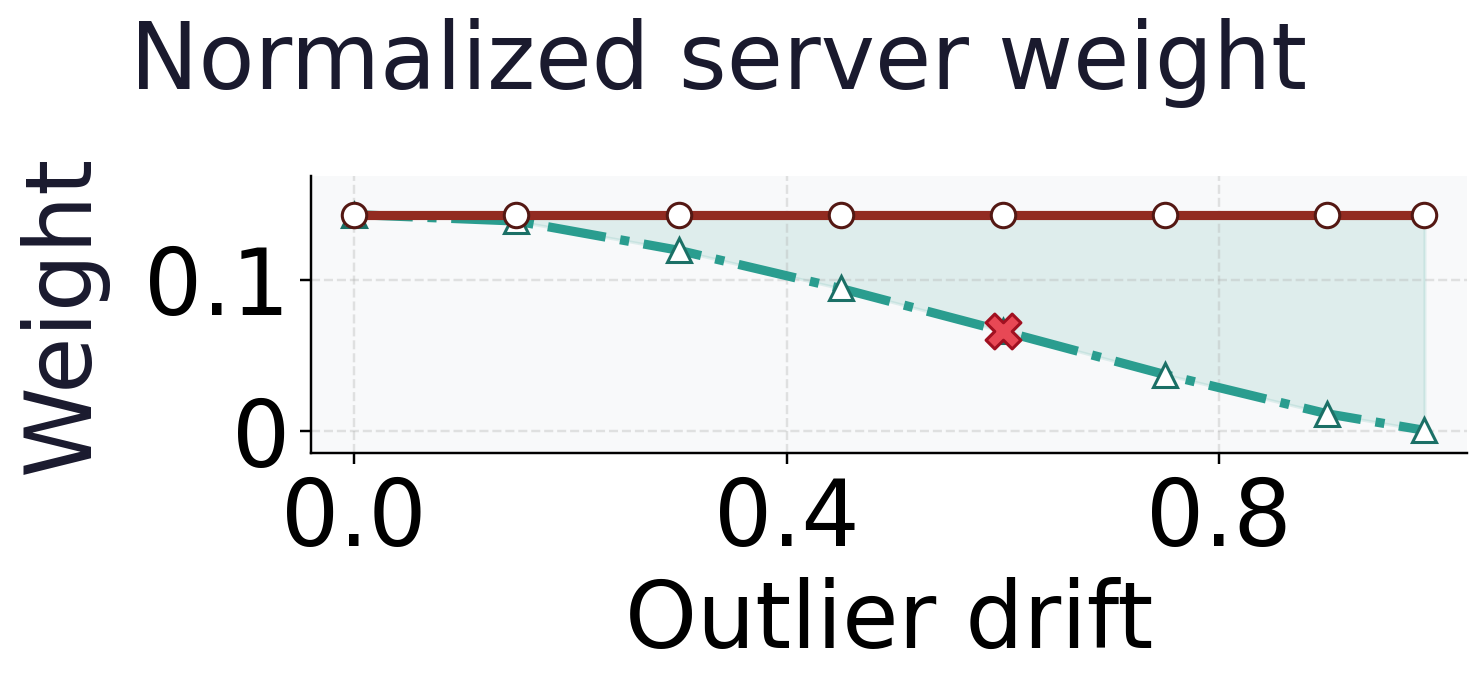
\includegraphics[keepaspectratio,width=0.98\linewidth,height=0.8\textheight,alt={Every configured drift: triangle/dash-dot variational weights, circle/solid naive weights; shaded gap is deterministic, not an interval.}]{../figures/bounded_influence.slide-weight-path.png}
\refstepcounter{figure}\label{fig:bounded-influence-slide-panel-1}
\end{figure}
\end{frame}

\begin{frame}{Variational aggregator (part 12)}
\begin{figure}
\centering

\includegraphics[keepaspectratio,width=0.98\linewidth,height=0.8\textheight,alt={Triangle/dash-dot: variational.
Circle/solid: naive fixed weight.
Shading: deterministic weight gap.}]{../figures/bounded_influence.slide-encoding.png}
\refstepcounter{figure}\label{fig:bounded-influence-slide-panel-2}
\end{figure}
\end{frame}

\begin{frame}{Variational aggregator (part 13)}
\begin{figure}
\centering
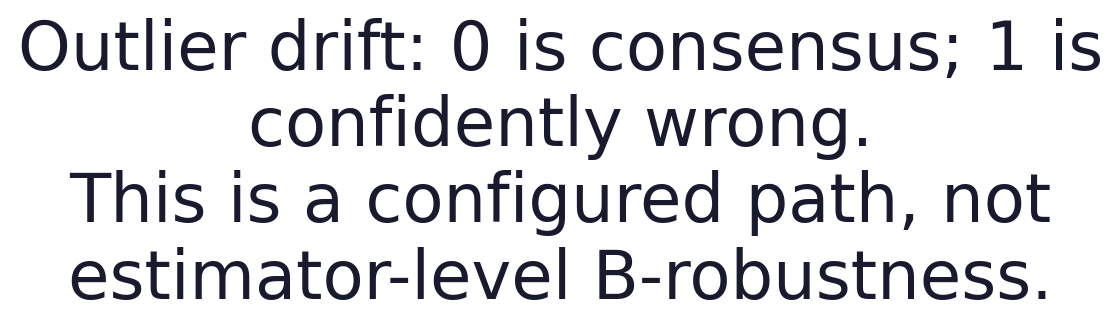
\includegraphics[keepaspectratio,width=0.98\linewidth,height=0.8\textheight,alt={Outlier drift: 0 is consensus; 1 is confidently wrong.
This is a configured path, not estimator-level B-robustness.}]{../figures/bounded_influence.slide-drift-key.png}
\refstepcounter{figure}\label{fig:bounded-influence-slide-panel-3}
\end{figure}
\end{frame}

\begin{frame}{Variational aggregator (part 14)}
\begin{figure}
\centering
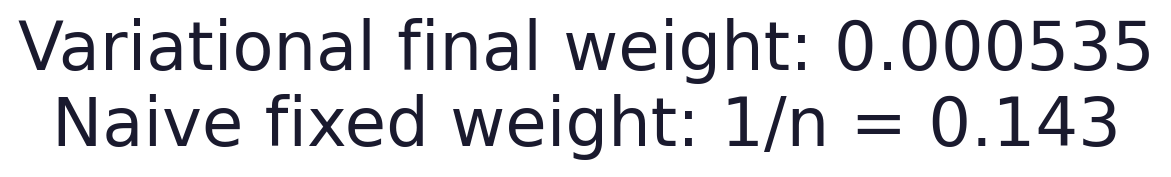
\includegraphics[keepaspectratio,width=0.98\linewidth,height=0.8\textheight,alt={Variational final weight: 0.000535
Naive fixed weight: 1/n = 0.143}]{../figures/bounded_influence.slide-endpoints.png}
\refstepcounter{figure}\label{fig:bounded-influence-slide-panel-4}
\end{figure}
\end{frame}

\begin{frame}{Variational aggregator (part 15)}
\begin{figure}
\centering
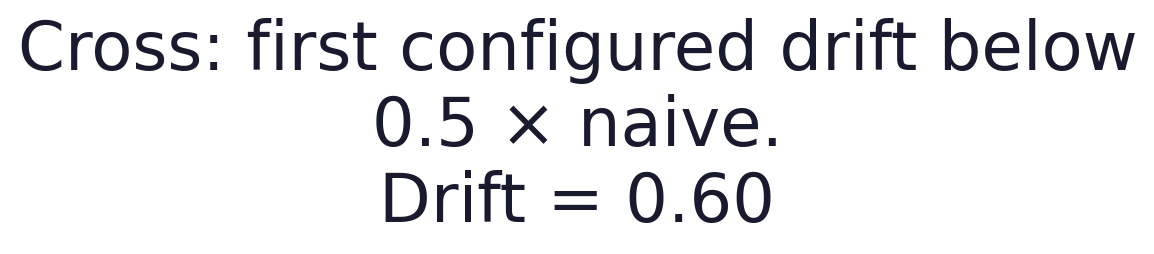
\includegraphics[keepaspectratio,width=0.98\linewidth,height=0.8\textheight,alt={Cross: first configured drift below 0.5 × naive.
Drift = 0.60}]{../figures/bounded_influence.slide-crossing.png}
\refstepcounter{figure}\label{fig:bounded-influence-slide-panel-5}
\end{figure}
\end{frame}

\begin{frame}{Variational aggregator (part 16)}
The honest trade is conservatism: because \(F\) carries the \(-H(q)\)
entropy term, its consensus is the maximum-entropy distribution
consistent with the weighted cross-entropies, deliberately flatter than
the product-of-experts.
\end{frame}

\begin{frame}{Variational aggregator (part 17)}
The variational aggregator therefore does \emph{not} win the
peak-accuracy verdict of sec.~7.5.2 --- that remains
the sharp heuristic's role --- and the two are reported as complements,
never conflated: rigor-with-conservatism on one side,
accuracy-without-an-objective on the other.
\end{frame}

\end{document}
